\documentclass[xcolor=dvipsnames]{beamer}
\usecolortheme[named=Brown]{structure}
\usetheme{default}
\setbeamertemplate{navigation symbols}{} 
\usepackage{tikz}
\usetikzlibrary{arrows,decorations.pathmorphing,backgrounds,positioning,fit}
\usetikzlibrary{datavisualization.formats.functions}
%     
%Here are some macro's saving time and labour:     
%     
\newcommand{\const}{\mbox{const}}      
\newcommand{\est}{\mbox{{\tiny est}}}      
\newcommand{\im}{\mbox{$\Im \mbox{m}$}}      
\newcommand{\obs}{\mbox{{\tiny obs}}}      
\newcommand{\otherwise}{\mbox{otherwise}}      
\newcommand{\real}{\mbox{$\Re \mbox{e}$}}      
\newcommand{\sign}{\mbox{sign}}      
\newcommand{\sinc}{\mbox{sinc}}      
%
\newcommand{\p}{\mbox{$\partial$}}      
\renewcommand{\d}{\mbox{$\partial$}}      
\newcommand{\w}{\mbox{$\omega$}}      
%
\newcommand{\AAA}{\mbox{\boldmath $A$}}   
\newcommand{\BB}{\mbox{\boldmath $B$}}     
\newcommand{\CC}{\mbox{\boldmath $C$}}     
\newcommand{\DD}{\mbox{\boldmath $D$}}     
\newcommand{\EE}{\mbox{\boldmath $E$}}     
\newcommand{\FF}{\mbox{\boldmath $F$}}   
\newcommand{\GG}{\mbox{\boldmath $G$}}   
\newcommand{\HH}{\mbox{\boldmath $H$}}   
\newcommand{\II}{\mbox{\boldmath $I$}}   
\newcommand{\JJ}{\mbox{\boldmath $J$}}   
\newcommand{\KK}{\mbox{\boldmath $K$}}   
\newcommand{\LL}{\mbox{\boldmath $L$}}   
\newcommand{\MM}{\mbox{\boldmath $M$}}   
\newcommand{\NN}{\mbox{\boldmath $N$}}   
\newcommand{\OO}{\mbox{\boldmath $O$}}   
\newcommand{\PP}{\mbox{\boldmath $P$}}   
\newcommand{\QQ}{\mbox{\boldmath $Q$}}   
\newcommand{\RR}{\mbox{\boldmath $R$}}   
\newcommand{\SSS}{\mbox{\boldmath $S$}}   
\newcommand{\TT}{\mbox{\boldmath $T$}}   
\newcommand{\UU}{\mbox{\boldmath $U$}}   
\newcommand{\VV}{\mbox{\boldmath $V$}}   
\newcommand{\WW}{\mbox{\boldmath $W$}}   
\newcommand{\XX}{\mbox{\boldmath $X$}}   
\newcommand{\YY}{\mbox{\boldmath $Y$}}   
\newcommand{\ZZ}{\mbox{\boldmath $Z$}}   
%
%\newcommand{\aaa}{\mbox{\boldmath $a$}}     
\newcommand{\bb}{\mbox{\boldmath $b$}}     
\newcommand{\cc}{\mbox{\boldmath $c$}}     
\newcommand{\dd}{\mbox{\boldmath $d$}}     
\newcommand{\ee}{\mbox{\boldmath $e$}}   
\newcommand{\ff}{\mbox{\boldmath $f$}}   
%\newcommand{\ggg}{\mbox{\boldmath $g$}}   
\newcommand{\hh}{\mbox{\boldmath $h$}}   
\newcommand{\ii}{\mbox{\boldmath $i$}}   
\newcommand{\jj}{\mbox{\boldmath $j$}}   
\newcommand{\kk}{\mbox{\boldmath $k$}}   
%\newcommand{\lll}{\mbox{\boldmath $l$}}   
\newcommand{\mm}{\mbox{\boldmath $m$}}   
\newcommand{\nn}{\mbox{\boldmath $n$}}   
\newcommand{\pp}{\mbox{\boldmath $p$}}   
\newcommand{\qq}{\mbox{\boldmath $q$}}   
\newcommand{\rr}{\mbox{\boldmath $r$}}   
%\newcommand{\sss}{\mbox{\boldmath $s$}}   
%\newcommand{\ttt}{\mbox{\boldmath $t$}}   
\newcommand{\uu}{\mbox{\boldmath $u$}}   
\newcommand{\vv}{\mbox{\boldmath $v$}}   
\newcommand{\ww}{\mbox{\boldmath $w$}}   
\newcommand{\xx}{\mbox{\boldmath $x$}}   
\newcommand{\yy}{\mbox{\boldmath $y$}}   
\newcommand{\zz}{\mbox{\boldmath $z$}}   
%
\newcommand{\balpha}{\mbox{\boldmath $\alpha$}}     
\newcommand{\bpsi}{\mbox{\boldmath $\psi$}}     
\newcommand{\bphi}{\mbox{\boldmath $\phi$}}     
\newcommand{\bbeta}{\mbox{\boldmath $\beta$}}     
\newcommand{\btheta}{\mbox{\boldmath $\theta$}}     
\newcommand{\bdelta}{\mbox{\boldmath $\delta$}}     
\newcommand{\bgamma}{\mbox{\boldmath $d$}}     
\newcommand{\bGamma}{\mbox{\boldmath $\Gamma$}}     
\newcommand{\bLambda}{\mbox{\boldmath $\Lambda$}}     
\newcommand{\bmu}{\mbox{\boldmath $\mu$}}     
\newcommand{\bnabla}{\mbox{\boldmath $\nabla$}}     
\newcommand{\brho}{\mbox{\boldmath $\rho$}}     
\newcommand{\bSigma}{\mbox{\boldmath $\Sigma$}}     
\newcommand{\bsigma}{\mbox{\boldmath $\sigma$}}     
\newcommand{\bxi}{\mbox{\boldmath $\xi$}}     
\newcommand{\bepsilon}{\mbox{\boldmath $\epsilon$}}     
\newcommand{\blambda}{\mbox{\boldmath $\lambda$}}     
\newcommand{\BLambda}{\mbox{\boldmath $\Lambda$}}     
%-------------------------------------%
%  \Appendix - a new appendix command %
%-------------------------------------%
%The appendix command is used as in
% \Appendix{A}{The wave equation as a matrix equation}
\newcommand {\Appendix}[1]{
              \section*{APPENDIX #1}
              \setcounter{equation}{0}
              \renewcommand{\theequation} 
              {A-\arabic{equation}}}
\newcommand {\Appendices}[2]{
              \section*{APPENDIX #1: #2 }
              \setcounter{equation}{0}
              \renewcommand{\theequation} 
              {#1-\arabic{equation}}}
%------------------------------------%
%    \aref - a new cite command.     % 
%------------------------------------%
\newcommand{\aref}[2]{\nocite{#1}#2} 
%----------------------------------------
%\eqref -an equation reference command
%----------------------------------------
%\newcommand{\eqref}[1]{(\ref{#1})}
%\newcommand{\eqref}[1]{\ref{#1}}

\usepackage{epsfig}
\begin{document}
%\setbeamercolor{titlelike}{fg=gray,bg=white}
%\setbeamercolor{itemize item}{fg=gray,bg=white}
%\setbeamercolor{enumerate item}{fg=gray,bg=white}
%\setbeamercolor{block title}{fg=black,bg=white}
%==============================================
\title{Reverse-time true amplitude migration}
\author{B. Arntsen}
\institute[NTNU]{
  NTNU\\
  Department of Petr. Techn. and Applied Geophysics\\
  \texttt{borge.arntsen@ntnu.no}
}
\date{Rose Meeting, April 2016}
\begin{frame}
 \titlepage
\end{frame}
%==============================================
%---------------------------------------------
\begin{frame}{Incorrect AVO behaviour}
%---------------------------------------------
\begin{figure}
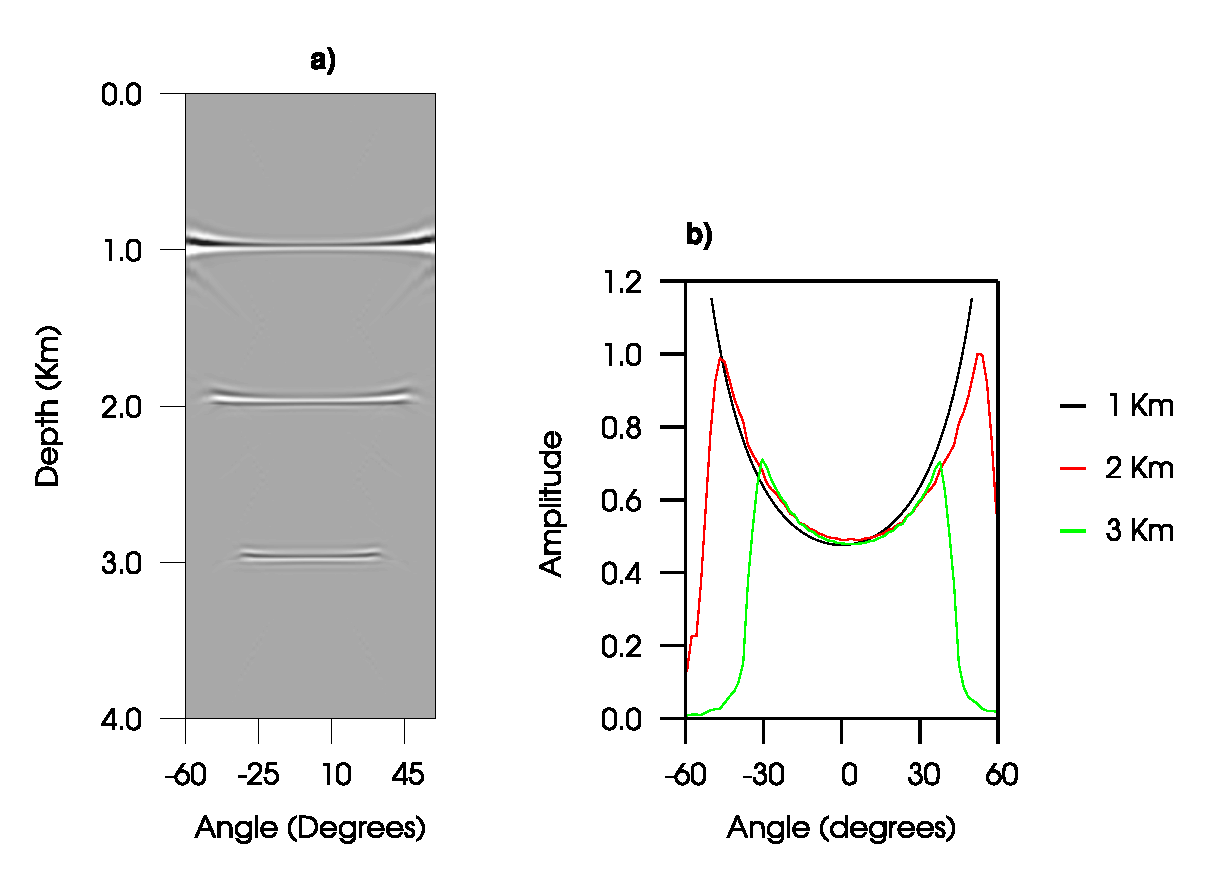
\epsfig{file=Fig/fig-4,width=10cm}
\end{figure}
(Arntsen et al 2013)
\end{frame}
%---------------------------------------------
\begin{frame}{Correct reflection coefficents}
%---------------------------------------------
%
\begin{figure}
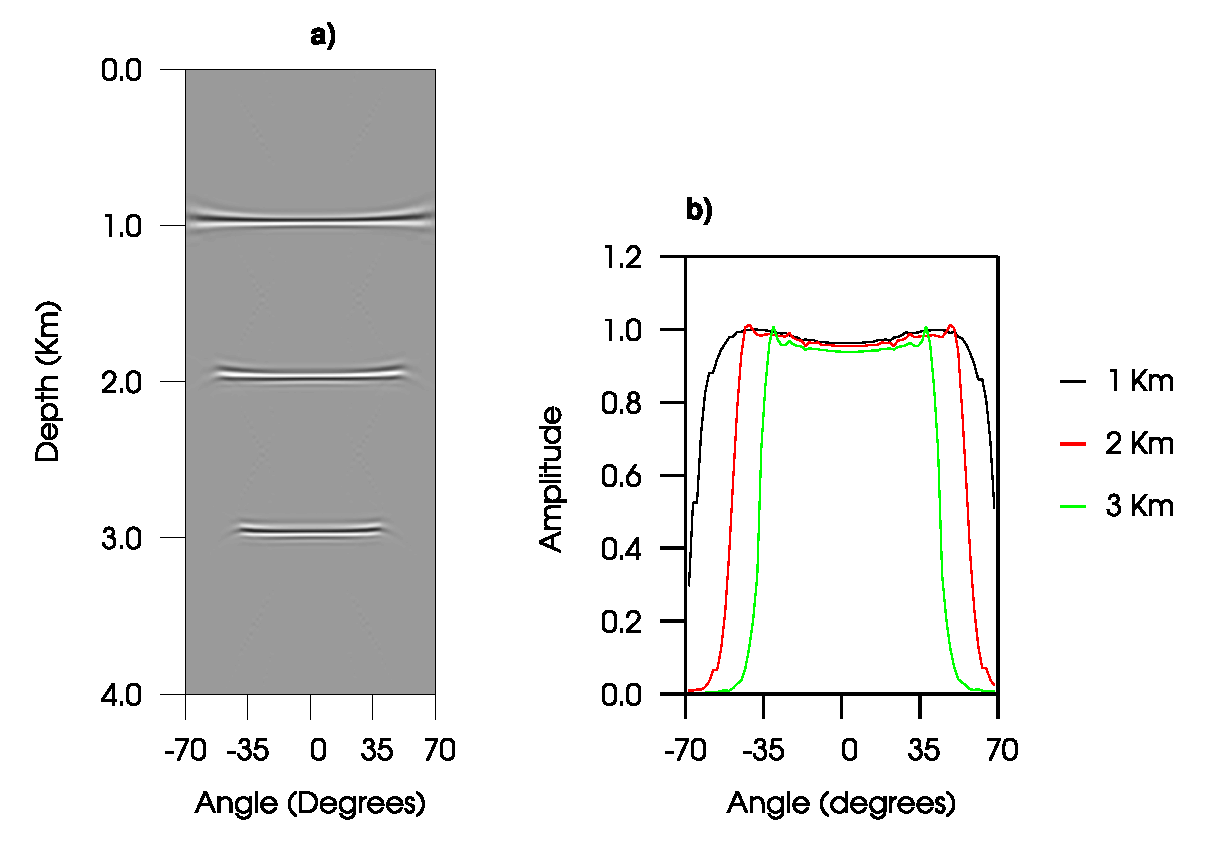
\epsfig{file=Fig/fig-2,width=10cm}
\end{figure}

(Arntsen et al. 2013)
\end{frame}
%-----------------------------------------
\begin{frame}{Overview}
%-----------------------------------------
\begin{enumerate}
  \item Introduction
  \item True Amplitude Imaging condition
  \item Numerical examples
  \item Conclusions
\end{enumerate}
\end{frame}
%-----------------------------------------
\begin{frame}{Introduction}
%-----------------------------------------
\begin{enumerate}
  \item AVO analysis important for exploration and reservoir characterization
  \item Output gathers from migration should ideally be equal to angle-dependent reflection coefficient
  \item The most commonly used imaging condition in Reverse-time migration gives gathers with incorrect angle-dependence
  \item Simple modification of Claerbouts (1971) imaging condition gives correct angle dependence
  \item Theoretically sound
\end{enumerate}
\end{frame}
%-----------------------------------------
\begin{frame}{Imaging condition}
%-----------------------------------------
\begin{figure}
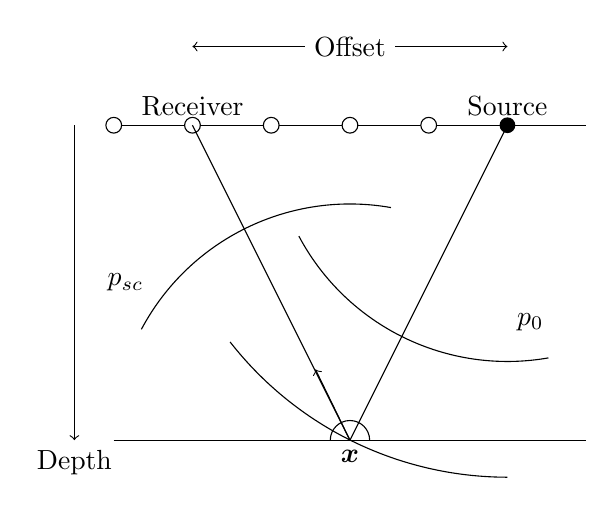
\begin{tikzpicture}[scale=1.0]
  \draw[->] (-0.5,4.0) -- (-0.5,0.0) node[below]{Depth} ;
  \draw[<->] (1.0,5.0) -- node[fill=white]{Offset} (5.0,5.0); 
  \draw (0.0,0.0) -- (6.0,0.0) ;
  \draw (0.0,4.0) -- (6.0,4.0) ;
  \fill (5.0,4.0) node[above]{Source} circle (0.1) ;
  \fill[white] (0.0,4.0) circle (0.1) ;
  \draw (0.0,4.0) circle (0.1) ;
  \fill[white](1.0,4.0) circle (0.1) ;
  \draw (1.0,4.0) node[above]{Receiver}circle (0.1) ;
  \fill[white] (2.0,4.0) circle (0.1) ;
  \draw (2.0,4.0) circle (0.1) ;
  \fill[white] (3.0,4.0) circle (0.1) ;
  \draw (3.0,4.0) circle (0.1) ;
  \fill[white] (4.0,4.0) circle (0.1) ;
  \draw (4.0,4.0) circle (0.1) ;
  \draw (5.0,4.0) -- (3.0,0.0) ;
  \draw (3.0,0.0) -- (1.0,4.0) ;
% Upgoing wave circle
  \draw (3,0) +(80:3) arc(80:152:3);
  \draw (3,0) +(0:0.25) arc(0:180:0.25);
  \draw (5,4) +(-80:3) arc(-80:-152:3);
  \draw (5,4) +(-90:4.47) arc(-90:-142:4.47);
  \draw (5.0,1.5) node[right]{$p_0$};
  \draw (0.5,2.0) node[left]{$p_{sc}$};
  \draw (3,0) node[below]{$\xx$};
  %\draw (3.4,0.125) node[below]{$\xx'$};
  \draw[->] (3,0)-- +(116:1);
\end{tikzpicture}
%\label{fig:si-1}
\end{figure}
\end{frame}
%-----------------------------------------
\begin{frame}{Imaging condition}
%-----------------------------------------
\begin{figure}
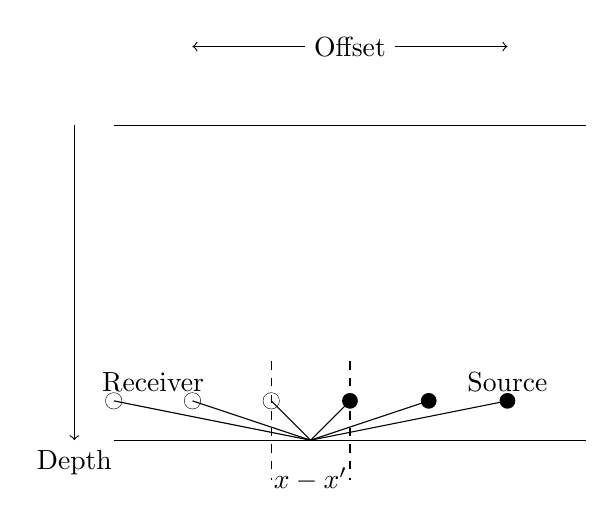
\begin{tikzpicture}[scale=1.0]
   \draw[->] (-0.5,4.0) -- (-0.5,0.0) node[below]{Depth} ;      %Depth axis 
   \draw[<->] (1.0,5.0) -- node[fill=white]{Offset} (5.0,5.0);  %Offset axis  
  \draw (0.0,4.0) -- (6.0,4.0) ;                               % Boundary at top
  \draw (0.0,0.0) -- (6.0,0.0) ;                               % Boundary at depth

  \fill (3.0,0.5) node[above]{} circle (0.1) ;           % Draw source
  \fill (4.0,0.5) node[above]{} circle (0.1) ;           % Draw source
  \fill (5.0,0.5) node[above]{Source} circle (0.1) ;     % Draw source text

  \draw (2.0,0.5) circle (0.1) ;             %Draw receiver
  \fill[white] (2.0,0.5) circle (0.1) ;

  \draw (1.0,0.5) circle (0.1) ;             %Draw receiver
  \fill[white] (1.0,0.5) circle (0.1) ;

  \draw (0.0,0.5) circle (0.1) ;             %Draw receiver
  \fill[white] (0.0,0.5) circle (0.1) ;
  \draw (0.5,0.5) node[above]{Receiver} ;    %Draw reeiver text 

  \draw (3.0,0.5) -- (2.5,0.0);              % Draw ray from source to midpoint
  \draw (4.0,0.5) -- (2.5,0.0);              % Draw ray from source to midpoint
  \draw (5.0,0.5) -- (2.5,0.0);              % Draw ray from source to midpoint

  \draw (2.0,0.5) -- (2.5,0.0);              % Draw ray from receiver to midpoint
  \draw (1.0,0.5) -- (2.5,0.0);              % Draw ray from receiver to midpoint
  \draw (0.0,0.5) -- (2.5,0.0);              % Draw ray from receiver to midpoint

  \draw[dashed] (2.0,1.0) -- (2.0,-0.5);     %Draw vertical dashed line
  \draw[dashed] (3.0,1.0) -- (3.0,-0.5);     %Draw vertical dashed line
  \draw (2.5,-0.5) node {$x-x'$};           % Draw equation

\end{tikzpicture}
%\label{fig:si-1}
\end{figure}
\end{frame}
%-----------------------------------------
\begin{frame}{Imaging condition}
%-----------------------------------------
\begin{figure}
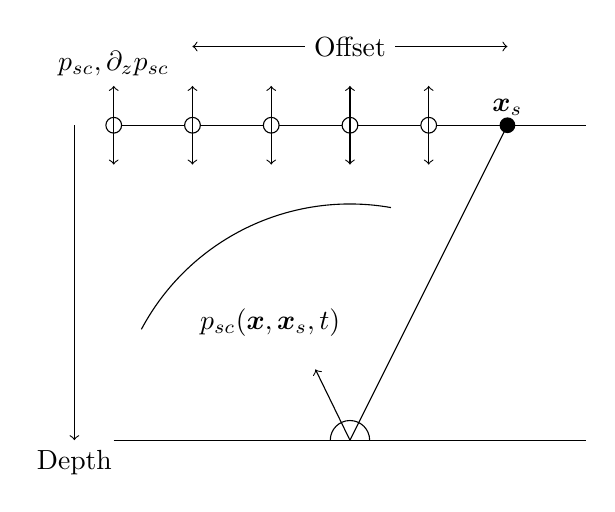
\begin{tikzpicture}[scale=1.0]
  \draw[->] (-0.5,4.0) -- (-0.5,0.0) node[below]{Depth} ;     %Draw Depth axis
  \draw[<->] (1.0,5.0) -- node[fill=white]{Offset} (5.0,5.0); %Draw offset axis 
  \draw (0.0,0.0) -- (6.0,0.0) ;  %Top boundary
  \draw (0.0,4.0) -- (6.0,4.0) ;  %Bottom boundary

  \fill (5.0,4.0) node[above]{$\xx_s$} circle (0.1) ; % Draw source

  \fill[white] (0.0,4.0) circle (0.1) ; %Draw receiver
  \draw (0.0,4.0) circle (0.1) ;
  \draw[->] (0.0,4.0) -- (0.0,4.5);
  \draw[->] (0.0,4.0) -- (0.0,3.5);
  \draw (0.0,4.5) node[above]{$p_{sc},\partial_z p_{sc}$};
  

  \fill[white](1.0,4.0) circle (0.1) ;
  \draw (1.0,4.0) node[above]{} circle (0.1) ;
  \draw[->] (1.0,4.0) -- (1.0,4.5);
  \draw[->] (1.0,4.0) -- (1.0,3.5);

  \fill[white] (2.0,4.0) circle (0.1) ;
  \draw (2.0,4.0) circle (0.1) ;
  \draw[->] (2.0,4.0) -- (2.0,4.5);
  \draw[->] (2.0,4.0) -- (2.0,3.5);

  \fill[white] (3.0,4.0) circle (0.1) ;
  \draw (3.0,4.0) circle (0.1) ;
  \draw[->] (3.0,4.0) -- (3.0,4.5);
  \draw[->] (3.0,4.0) -- (3.0,3.5);

  \fill[white] (4.0,4.0) circle (0.1) ;
  \draw (4.0,4.0) circle (0.1) ;
  \draw[->] (4.0,4.0) -- (4.0,4.5);
  \draw[->] (4.0,4.0) -- (4.0,3.5);

  \draw[->] (3,0)-- +(116:1);
  \draw (3,0) +(0:0.25) arc(0:180:0.25);
  \draw (3,0) +(80:3) arc(80:152:3);
  \draw (3.0,1.5) node[left]{$p_{sc}(\xx,\xx_s,t)$};


  \draw (5.0,4.0) -- (3.0,0.0) ;
  %\draw (3.0,0.0) -- (1.0,4.0) ;
\end{tikzpicture}
%\label{fig:si-1}
\end{figure}
\end{frame}
%-----------------------------------------
\begin{frame}{Imaging condition}
%-----------------------------------------
\begin{figure}
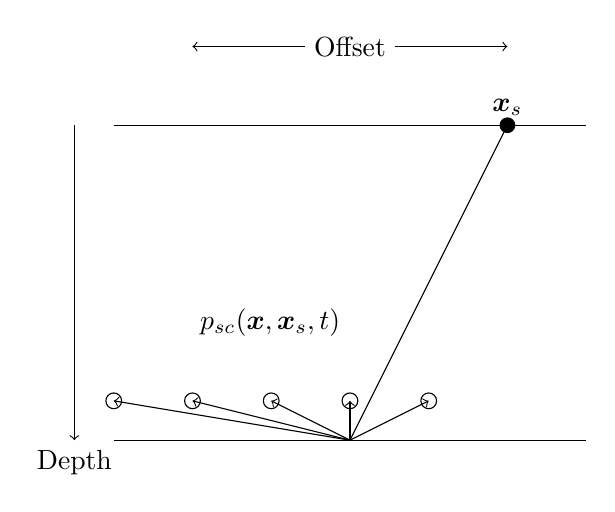
\begin{tikzpicture}[scale=1.0]
  \draw[->] (-0.5,4.0) -- (-0.5,0.0) node[below]{Depth} ;     %Draw Depth axis
  \draw[<->] (1.0,5.0) -- node[fill=white]{Offset} (5.0,5.0); %Draw offset axis 
  \draw (0.0,0.0) -- (6.0,0.0) ;  %Top boundary
  \draw (0.0,4.0) -- (6.0,4.0) ;  %Bottom boundary

  \fill (5.0,4.0) node[above]{$\xx_s$} circle (0.1) ; % Draw source

  \fill[white] (0.0,0.5) circle (0.1) ; %Draw receiver
  \draw (0.0,0.5) circle (0.1) ;
  

  \fill[white](1.0,0.5) circle (0.1) ;
  \draw (1.0,0.5) node[above]{} circle (0.1) ;

  \fill[white] (2.0,0.5) circle (0.1) ;
  \draw (2.0,0.5) circle (0.1) ;

  \fill[white] (3.0,0.5) circle (0.1) ;
  \draw (3.0,0.5) circle (0.1) ;

  \fill[white] (4.0,0.5) circle (0.1) ;
  \draw (4.0,0.5) circle (0.1) ;

  \draw[->] (3,0)-- (0.0,0.5);
  \draw[->] (3,0)-- (1.0,0.5);
  \draw[->] (3,0)-- (2.0,0.5);
  \draw[->] (3,0)-- (3.0,0.5);
  \draw[->] (3,0)-- (4.0,0.5);
%  \draw (3,0) +(0:0.25) arc(0:180:0.25);
%  \draw (3,0) +(80:3) arc(80:152:3);
  \draw (3.0,1.5) node[left]{$p_{sc}(\xx,\xx_s,t)$};


  \draw (5.0,4.0) -- (3.0,0.0) ;
  %\draw (3.0,0.0) -- (1.0,4.0) ;
\end{tikzpicture}
%\label{fig:si-1}
\end{figure}
\end{frame}
%-----------------------------------------
\begin{frame}{Imaging condition}
%-----------------------------------------
\begin{figure}
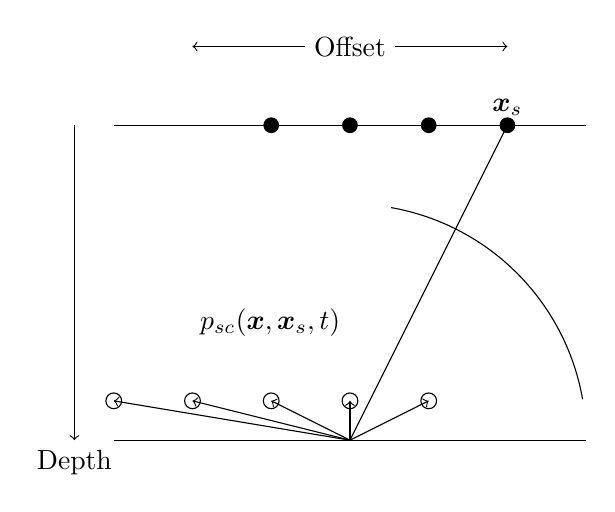
\begin{tikzpicture}[scale=1.0]
  \draw[->] (-0.5,4.0) -- (-0.5,0.0) node[below]{Depth} ;     %Draw Depth axis
  \draw[<->] (1.0,5.0) -- node[fill=white]{Offset} (5.0,5.0); %Draw offset axis 
  \draw (0.0,0.0) -- (6.0,0.0) ;  %Top boundary
  \draw (0.0,4.0) -- (6.0,4.0) ;  %Bottom boundary

  \fill (5.0,4.0) node[above]{$\xx_s$} circle (0.1) ; % Draw source
  \fill (4.0,4.0) node[above]{} circle (0.1) ; % Draw source
  \fill (3.0,4.0) node[above]{} circle (0.1) ; % Draw source
  \fill (2.0,4.0) node[above]{} circle (0.1) ; % Draw source

  \fill[white] (0.0,0.5) circle (0.1) ; %Draw receiver
  \draw (0.0,0.5) circle (0.1) ;
  

  \fill[white](1.0,0.5) circle (0.1) ;
  \draw (1.0,0.5) node[above]{} circle (0.1) ;

  \fill[white] (2.0,0.5) circle (0.1) ;
  \draw (2.0,0.5) circle (0.1) ;

  \fill[white] (3.0,0.5) circle (0.1) ;
  \draw (3.0,0.5) circle (0.1) ;

  \fill[white] (4.0,0.5) circle (0.1) ;
  \draw (4.0,0.5) circle (0.1) ;

  \draw[->] (3,0)-- (0.0,0.5);
  \draw[->] (3,0)-- (1.0,0.5);
  \draw[->] (3,0)-- (2.0,0.5);
  \draw[->] (3,0)-- (3.0,0.5);
  \draw[->] (3,0)-- (4.0,0.5);
%  \draw (3,0) +(0:0.25) arc(0:180:0.25);
%  \draw (3,0) +(80:3) arc(80:152:3);
  \draw (3.0,1.5) node[left]{$p_{sc}(\xx,\xx_s,t)$};
\draw (3,0) +(80:3) arc(80:10:3);


  \draw (5.0,4.0) -- (3.0,0.0) ;
  %\draw (3.0,0.0) -- (1.0,4.0) ;
\end{tikzpicture}
%\label{fig:si-1}
\end{figure}
\end{frame}
%-----------------------------------------
\begin{frame}{Imaging condition}
%-----------------------------------------
%
New imaging condition for multicomponent streamer data:
\begin{eqnarray}
  r(\xx,\xx')=
    \sum_{\xx_s}\int dt\, \d_z p_0(\xx,\xx_s,t)p_{sc}(\xx',\xx_s,t)\nonumber\\ 
    -\sum_{\xx_s} \int dt\, p_0 (\xx,\xx_s,t)\d_z p_{sc}(\xx',\xx_s,t)
\end{eqnarray}

New imaging condition for conventional streamer data:
%
\begin{eqnarray}
  r(\xx,\xx')= 
    \sum_{\xx_s} \int dt\, \d_z p_0(\xx,\xx_s,t) p_{sc}(\xx',\xx_s,t)
\end{eqnarray}
%
Old imaging condition: (Rickett and Sava, 2002)
\begin{eqnarray}
    r_{c}(\xx,\xx')=\sum_{\xx_s}\int dt\, p_0(\xx,\xx_s,t)p_{sc}(\xx',\xx_s,t) 
\end{eqnarray}
\end{frame}
%-----------------------------------------
\begin{frame}{Imaging condition}
%-----------------------------------------
\begin{figure}
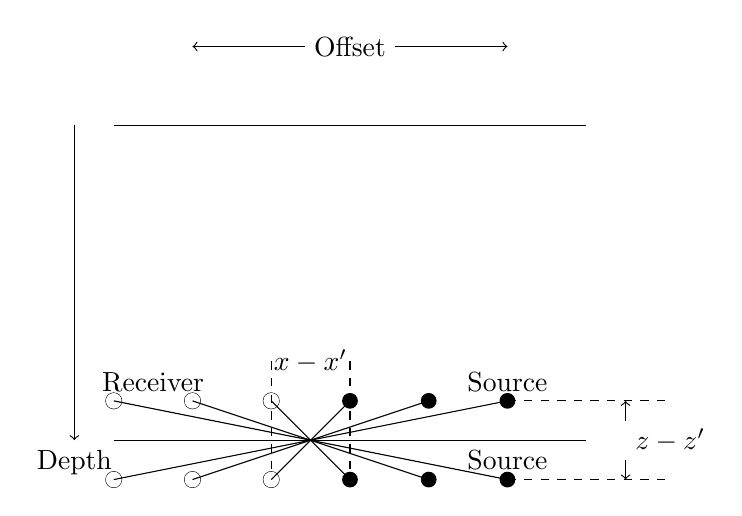
\begin{tikzpicture}[scale=1.0]
   \draw[->] (-0.5,4.0) -- (-0.5,0.0) node[below]{Depth} ;      %Depth axis 
   \draw[<->] (1.0,5.0) -- node[fill=white]{Offset} (5.0,5.0);  %Offset axis  
  \draw (0.0,4.0) -- (6.0,4.0) ;                               % Boundary at top
  \draw (0.0,0.0) -- (6.0,0.0) ;                               % Boundary at depth

  \fill (3.0,0.5) node[above]{} circle (0.1) ;           % Draw source
  \fill (4.0,0.5) node[above]{} circle (0.1) ;           % Draw source
  \fill (5.0,0.5) node[above]{Source} circle (0.1) ;     % Draw source text

  \draw (2.0,0.5) circle (0.1) ;             %Draw receiver
  \fill[white] (2.0,0.5) circle (0.1) ;

  \draw (1.0,0.5) circle (0.1) ;             %Draw receiver
  \fill[white] (1.0,0.5) circle (0.1) ;

  \draw (0.0,0.5) circle (0.1) ;             %Draw receiver
  \fill[white] (0.0,0.5) circle (0.1) ;
  \draw (0.5,0.5) node[above]{Receiver} ;    %Draw reeiver text 

  \draw (3.0,0.5) -- (2.5,0.0);              % Draw ray from source to midpoint
  \draw (4.0,0.5) -- (2.5,0.0);              % Draw ray from source to midpoint
  \draw (5.0,0.5) -- (2.5,0.0);              % Draw ray from source to midpoint

  \draw (2.0,0.5) -- (2.5,0.0);              % Draw ray from receiver to midpoint
  \draw (1.0,0.5) -- (2.5,0.0);              % Draw ray from receiver to midpoint
  \draw (0.0,0.5) -- (2.5,0.0);              % Draw ray from receiver to midpoint

  \draw[dashed] (2.0,1.0) -- (2.0,-0.5);     %Draw vertical dashed line
  \draw[dashed] (3.0,1.0) -- (3.0,-0.5);     %Draw vertical dashed line
  \draw (2.5,1.0) node {$x-x'$};           % Draw equation
  \draw[dashed] (5.0,0.5) -- (7.0,0.5);     %Draw vertical dashed line
  \draw[dashed] (5.0,-0.5) -- (7.0,-0.5);     %Draw vertical dashed line
  \draw (6.5,0.0) node[right]{$z-z'$};           % Draw equation
  \draw[->] (6.5,0.25) -- (6.5,0.5);
  \draw[->] (6.5,-0.25) -- (6.5,-0.5);



  \fill (3.0,-0.5) node[above]{} circle (0.1) ;           % Draw source
  \fill (4.0,-0.5) node[above]{} circle (0.1) ;           % Draw source
  \fill (5.0,-0.5) node[above]{Source} circle (0.1) ;     % Draw source text

  \draw (2.0,-0.5) circle (0.1) ;             %Draw receiver
  \fill[white] (2.0,-0.5) circle (0.1) ;

  \draw (1.0,-0.5) circle (0.1) ;             %Draw receiver
  \fill[white] (1.0,-0.5) circle (0.1) ;

  \draw (0.0,-0.5) circle (0.1) ;             %Draw receiver
  \fill[white] (0.0,-0.5) circle (0.1) ;
  %\draw (0.5,0.5) node[above]{Receiver} ;    %Draw reeiver text 

  \draw (3.0,-0.5) -- (2.5,0.0);              % Draw ray from source to midpoint
  \draw (4.0,-0.5) -- (2.5,0.0);              % Draw ray from source to midpoint
  \draw (5.0,-0.5) -- (2.5,0.0);              % Draw ray from source to midpoint

  \draw (2.0,-0.5) -- (2.5,0.0);              % Draw ray from receiver to midpoint
  \draw (1.0,-0.5) -- (2.5,0.0);              % Draw ray from receiver to midpoint
  \draw (0.0,-0.5) -- (2.5,0.0);              % Draw ray from receiver to midpoint
\end{tikzpicture}
\end{figure}
\end{frame}
%-----------------------------------------
\begin{frame}{Imaging condition}
%-----------------------------------------
%
Plane wave reflection coefficient:
\begin{eqnarray}
  r(\xx,\kk_h, z)=\int d\hh\,\exp(i\kk_h \cdot \hh) r(\xx,\hh=\xx-\xx')
\end{eqnarray}
\end{frame}
%
%-----------------------------------------
\begin{frame}{Numerical example}
%-----------------------------------------
%
\begin{figure}
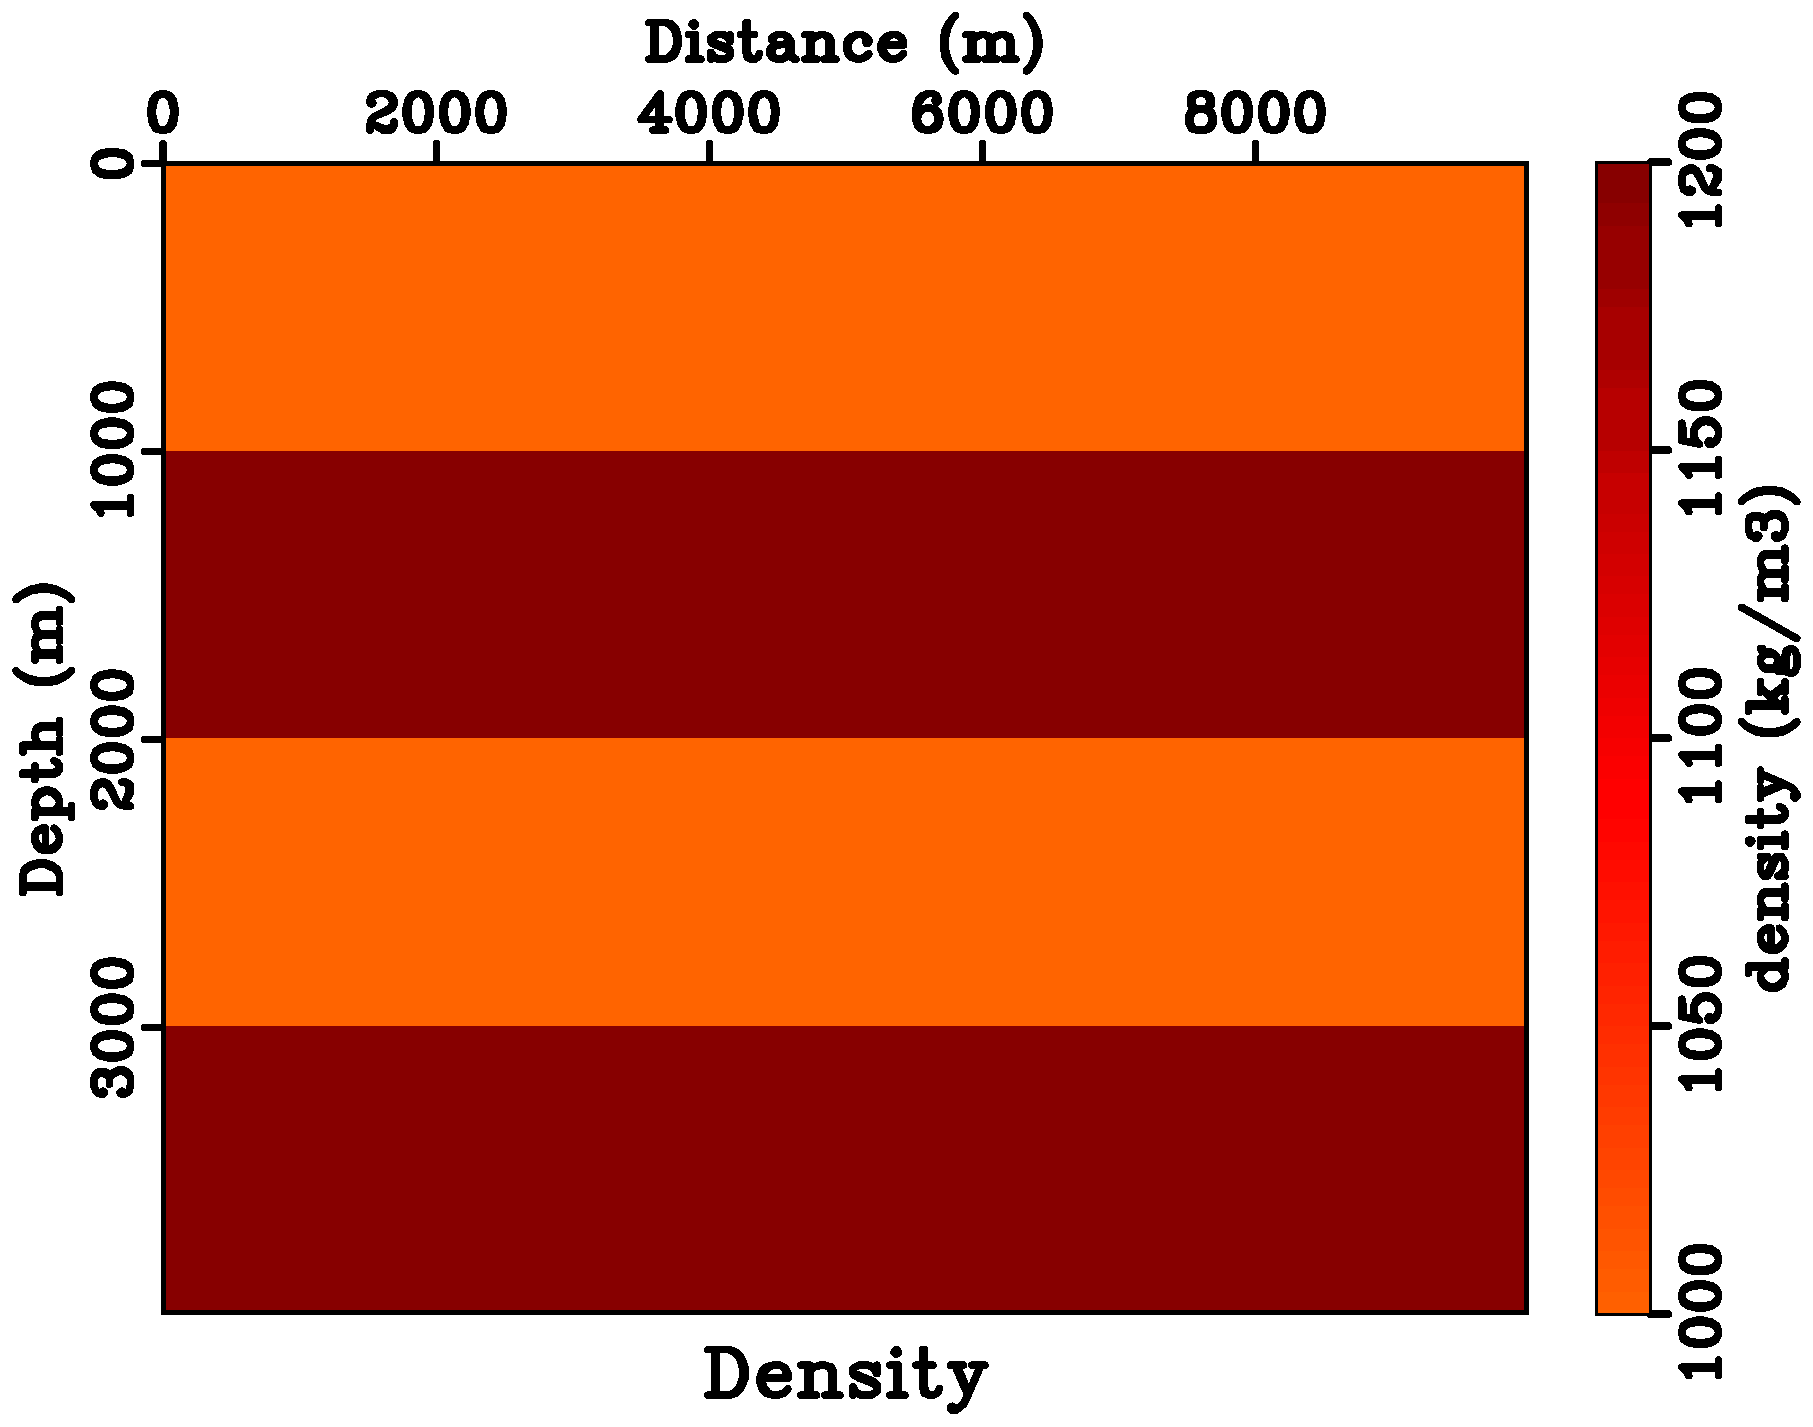
\epsfig{file=Fig/rho-1,width=10cm}
\end{figure}
\end{frame}
%-----------------------------------------
\begin{frame}{Numerical example}
%-----------------------------------------
%
\begin{figure}
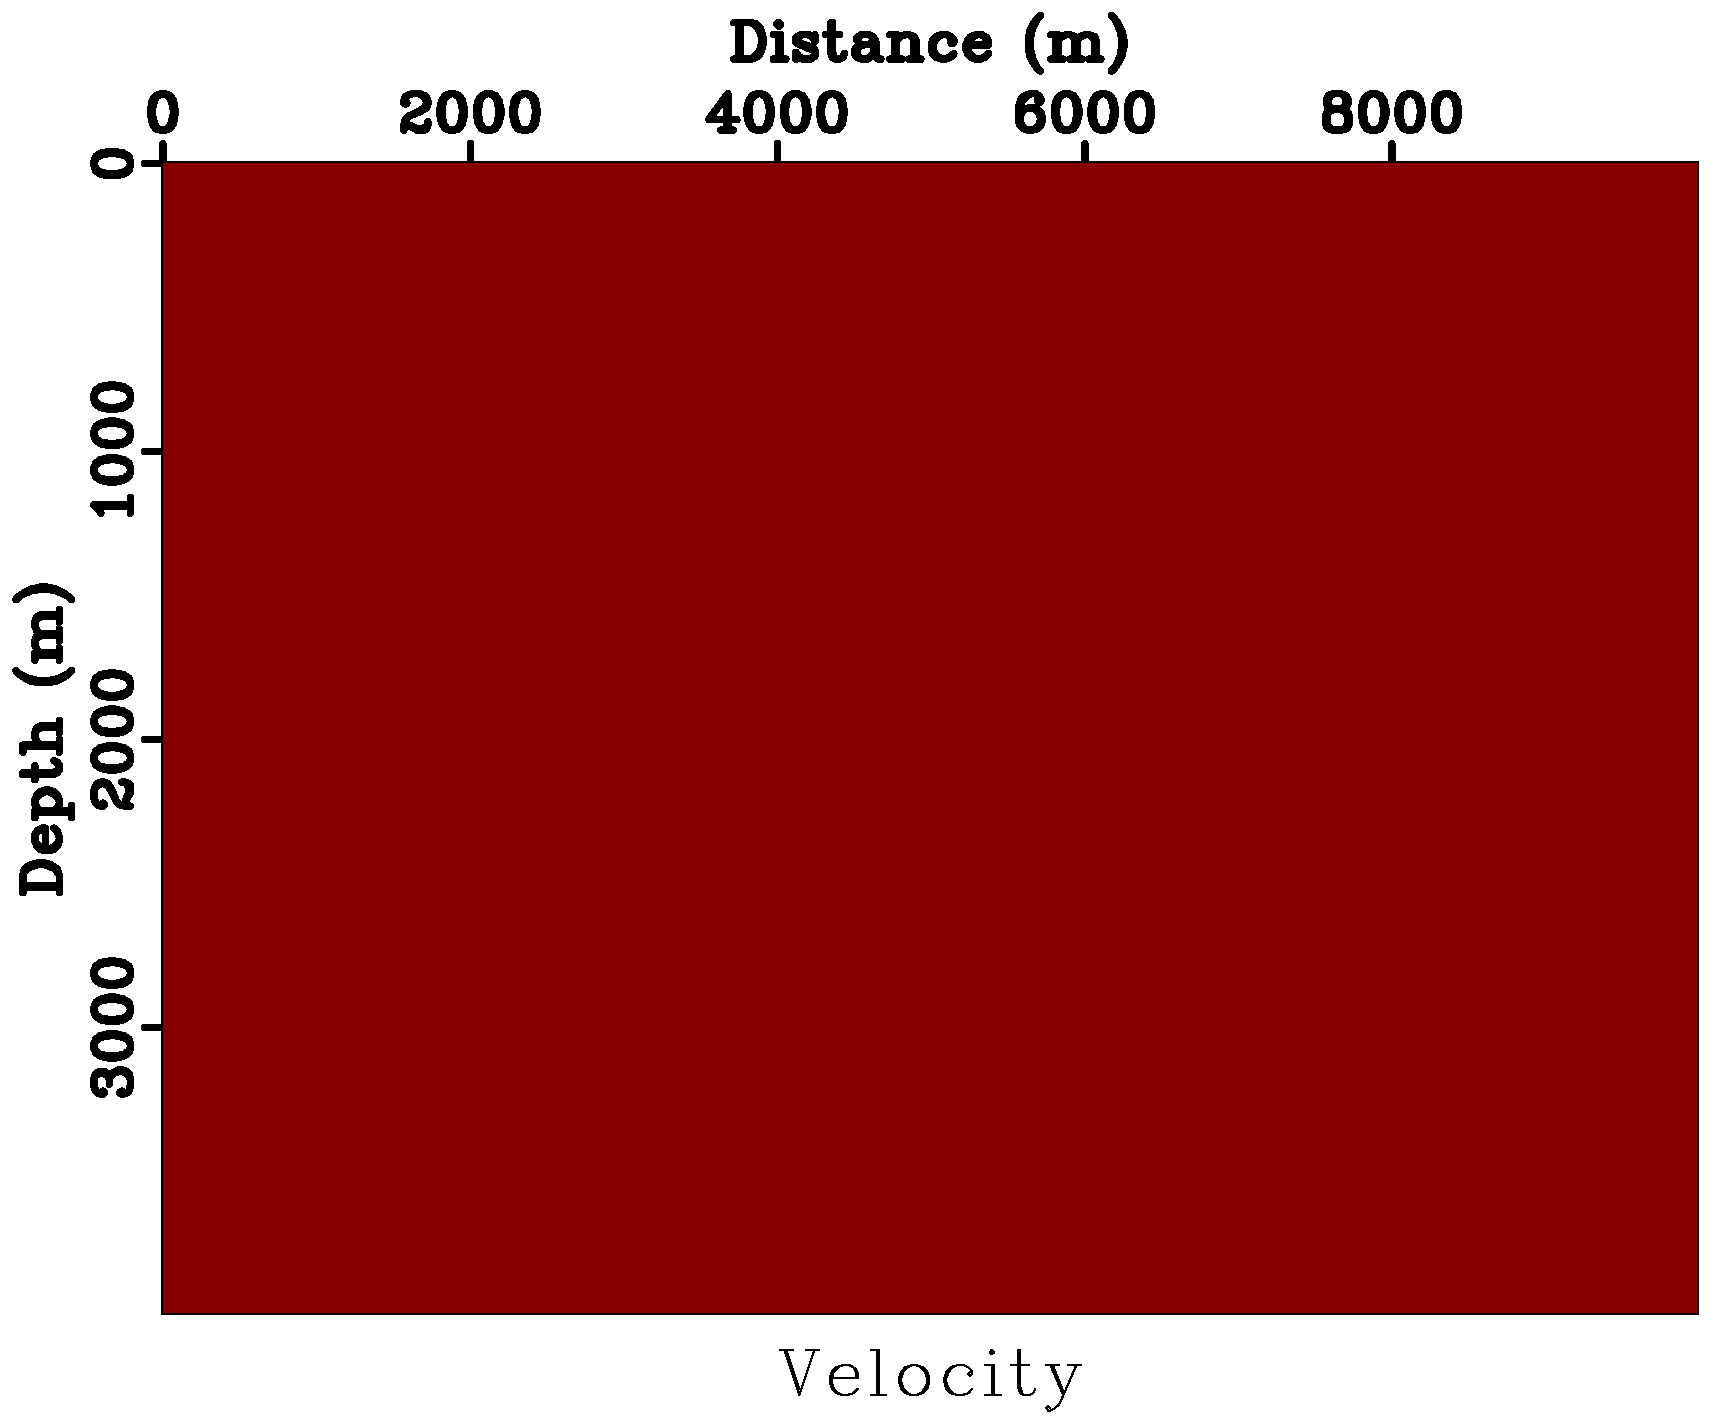
\epsfig{file=Fig/vp-1,width=10cm}
\end{figure}
\end{frame}
%-----------------------------------------
\begin{frame}{Numerical example}
%-----------------------------------------
%
\begin{figure}
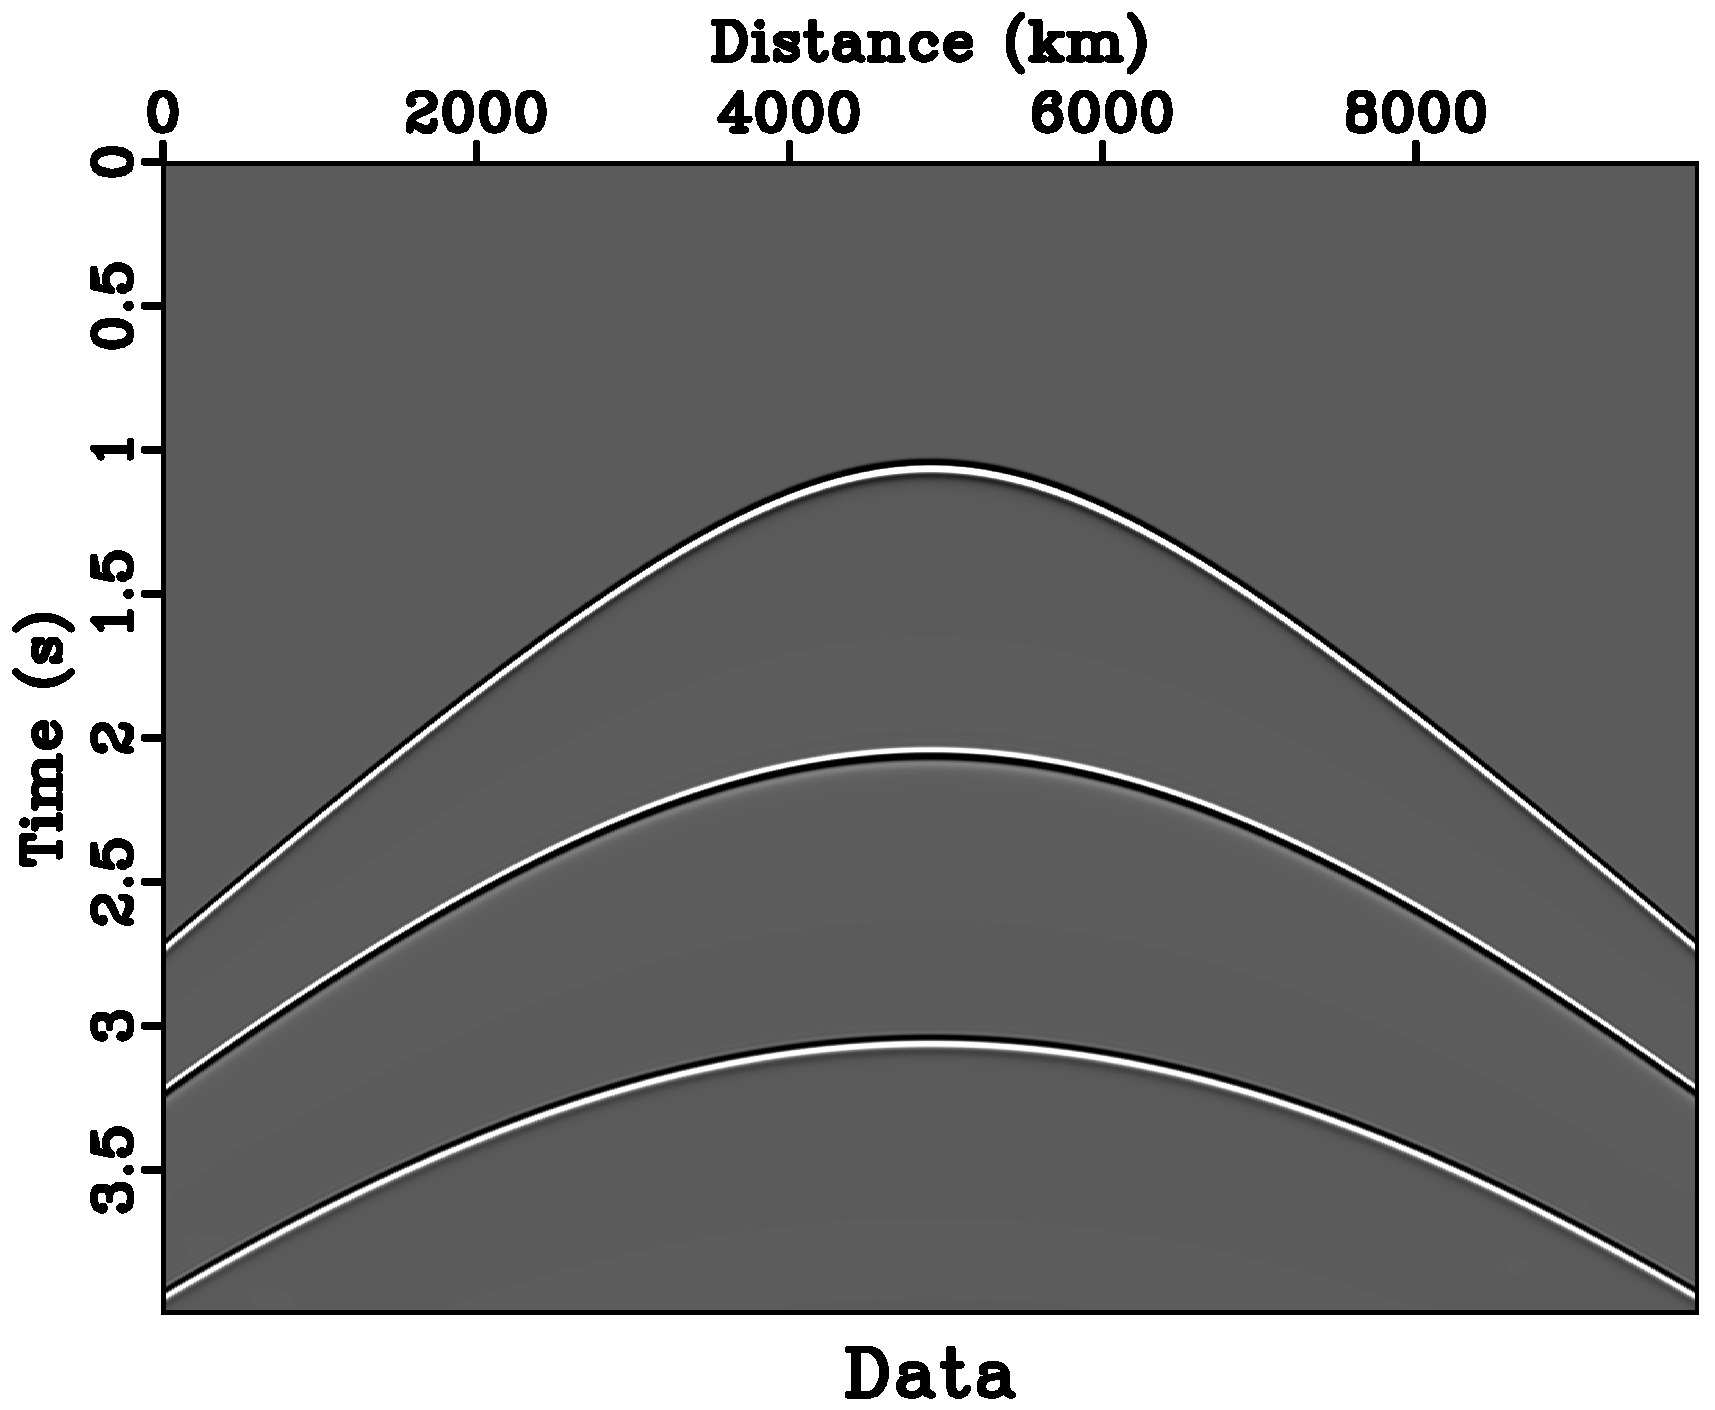
\epsfig{file=Fig/data-1-scatter,width=10cm}
\end{figure}
\end{frame}
%-----------------------------------------
\begin{frame}{Imaging condition}
%-----------------------------------------
Data at depth:
\begin{figure}
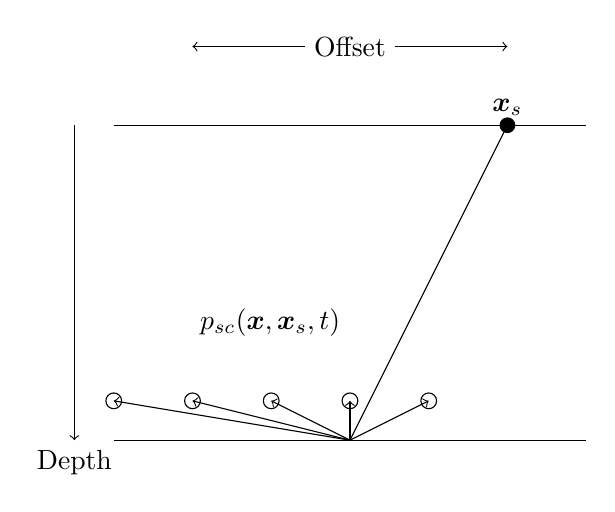
\begin{tikzpicture}[scale=1.0]
  \draw[->] (-0.5,4.0) -- (-0.5,0.0) node[below]{Depth} ;     %Draw Depth axis
  \draw[<->] (1.0,5.0) -- node[fill=white]{Offset} (5.0,5.0); %Draw offset axis 
  \draw (0.0,0.0) -- (6.0,0.0) ;  %Top boundary
  \draw (0.0,4.0) -- (6.0,4.0) ;  %Bottom boundary

  \fill (5.0,4.0) node[above]{$\xx_s$} circle (0.1) ; % Draw source

  \fill[white] (0.0,0.5) circle (0.1) ; %Draw receiver
  \draw (0.0,0.5) circle (0.1) ;
  

  \fill[white](1.0,0.5) circle (0.1) ;
  \draw (1.0,0.5) node[above]{} circle (0.1) ;

  \fill[white] (2.0,0.5) circle (0.1) ;
  \draw (2.0,0.5) circle (0.1) ;

  \fill[white] (3.0,0.5) circle (0.1) ;
  \draw (3.0,0.5) circle (0.1) ;

  \fill[white] (4.0,0.5) circle (0.1) ;
  \draw (4.0,0.5) circle (0.1) ;

  \draw[->] (3,0)-- (0.0,0.5);
  \draw[->] (3,0)-- (1.0,0.5);
  \draw[->] (3,0)-- (2.0,0.5);
  \draw[->] (3,0)-- (3.0,0.5);
  \draw[->] (3,0)-- (4.0,0.5);
%  \draw (3,0) +(0:0.25) arc(0:180:0.25);
%  \draw (3,0) +(80:3) arc(80:152:3);
  \draw (3.0,1.5) node[left]{$p_{sc}(\xx,\xx_s,t)$};


  \draw (5.0,4.0) -- (3.0,0.0) ;
  %\draw (3.0,0.0) -- (1.0,4.0) ;
\end{tikzpicture}
%\label{fig:si-1}
\end{figure}
\end{frame}
%-----------------------------------------
\begin{frame}{Numerical example}
%-----------------------------------------
$p_{sc}(\xx,\xx_s,t)$ at depth of 1000 m.
%
\begin{figure}
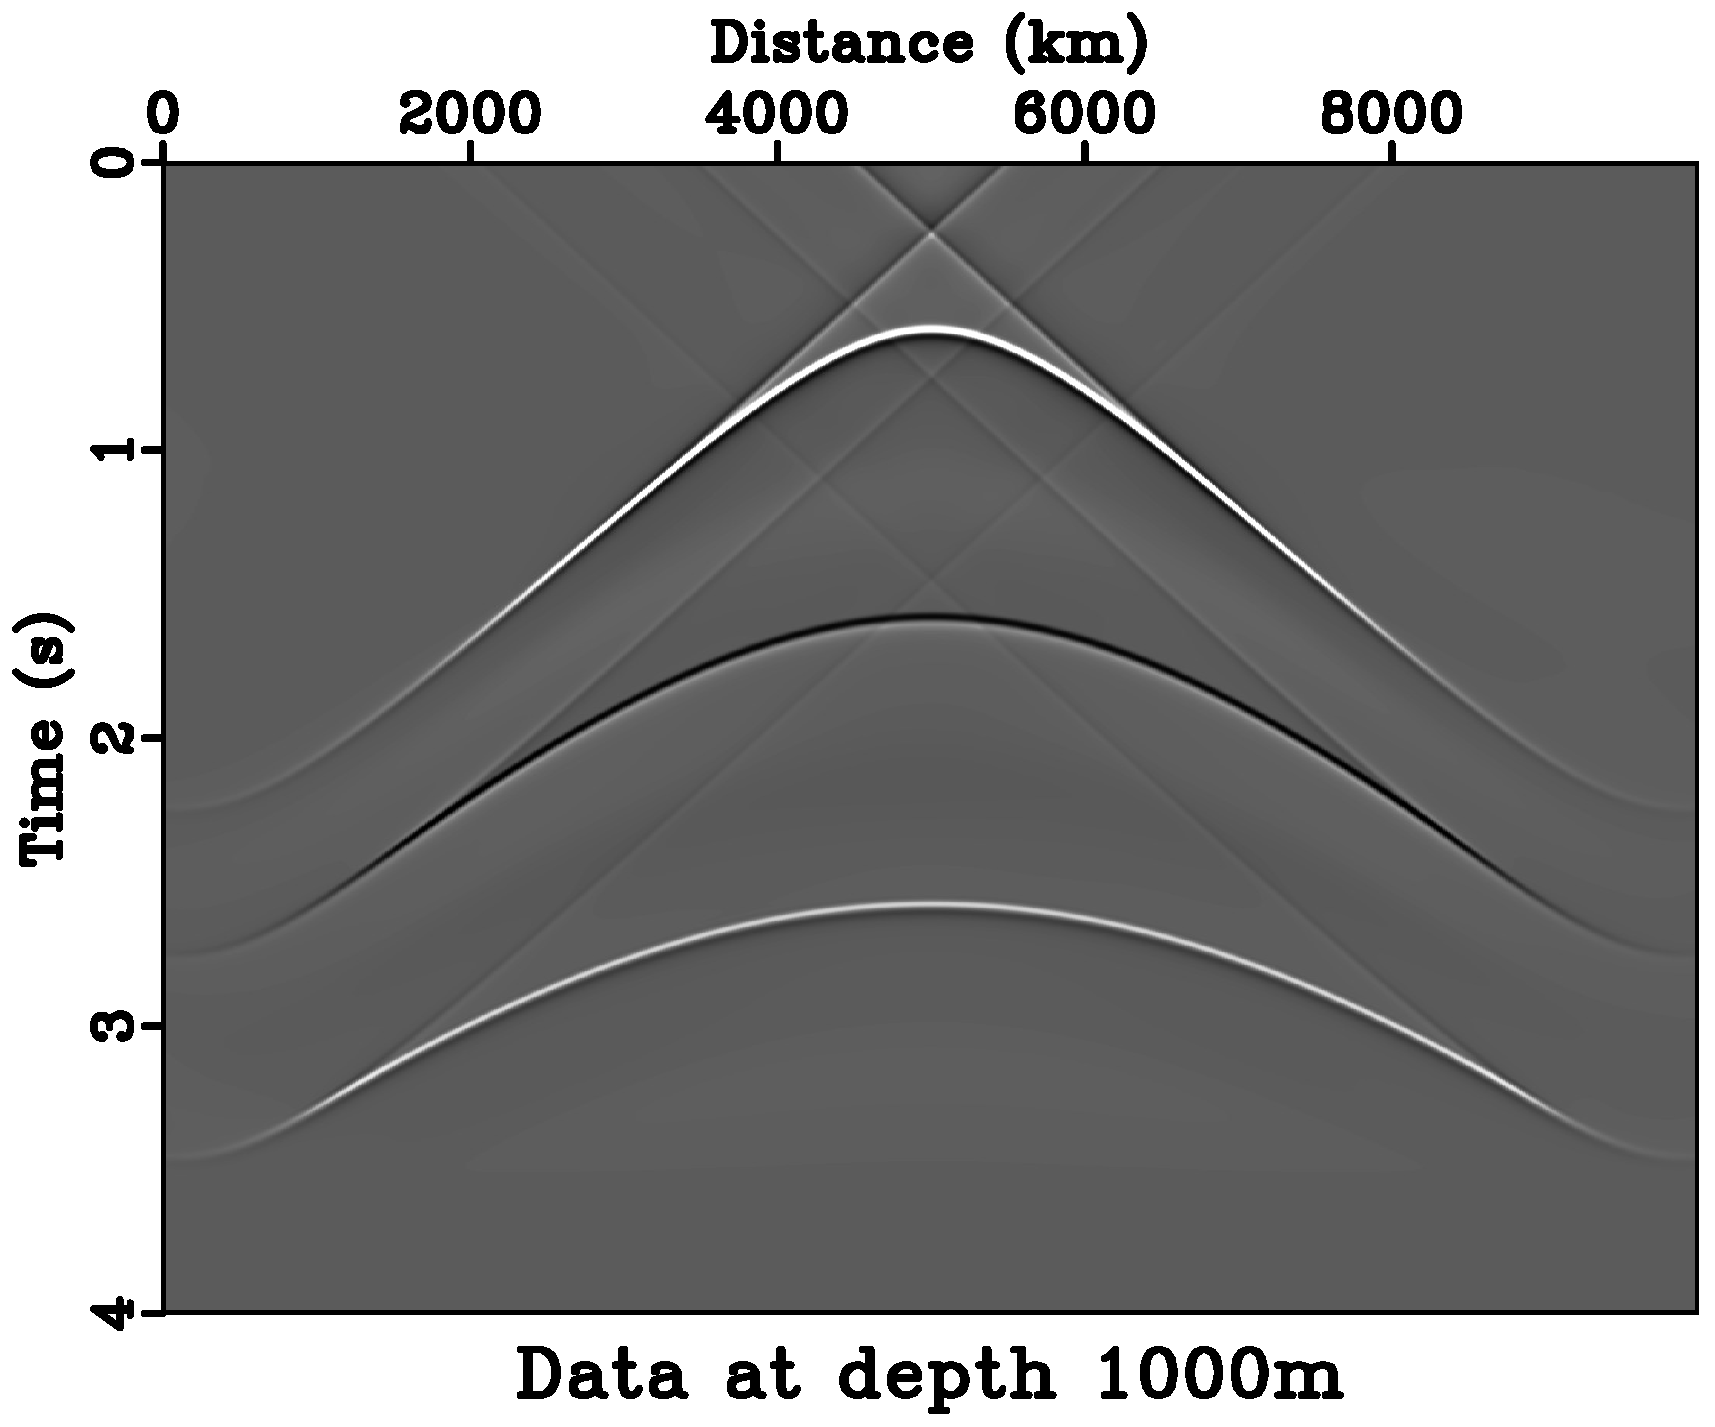
\epsfig{file=Fig/data-1-scatter-redat,width=8cm}
\end{figure}
\end{frame}
%-----------------------------------------
\begin{frame}{Numerical example}
%-----------------------------------------
$\hat{p}_0(\xx,\xx_s,t)$ at depth of 1000 m
%
\begin{figure}
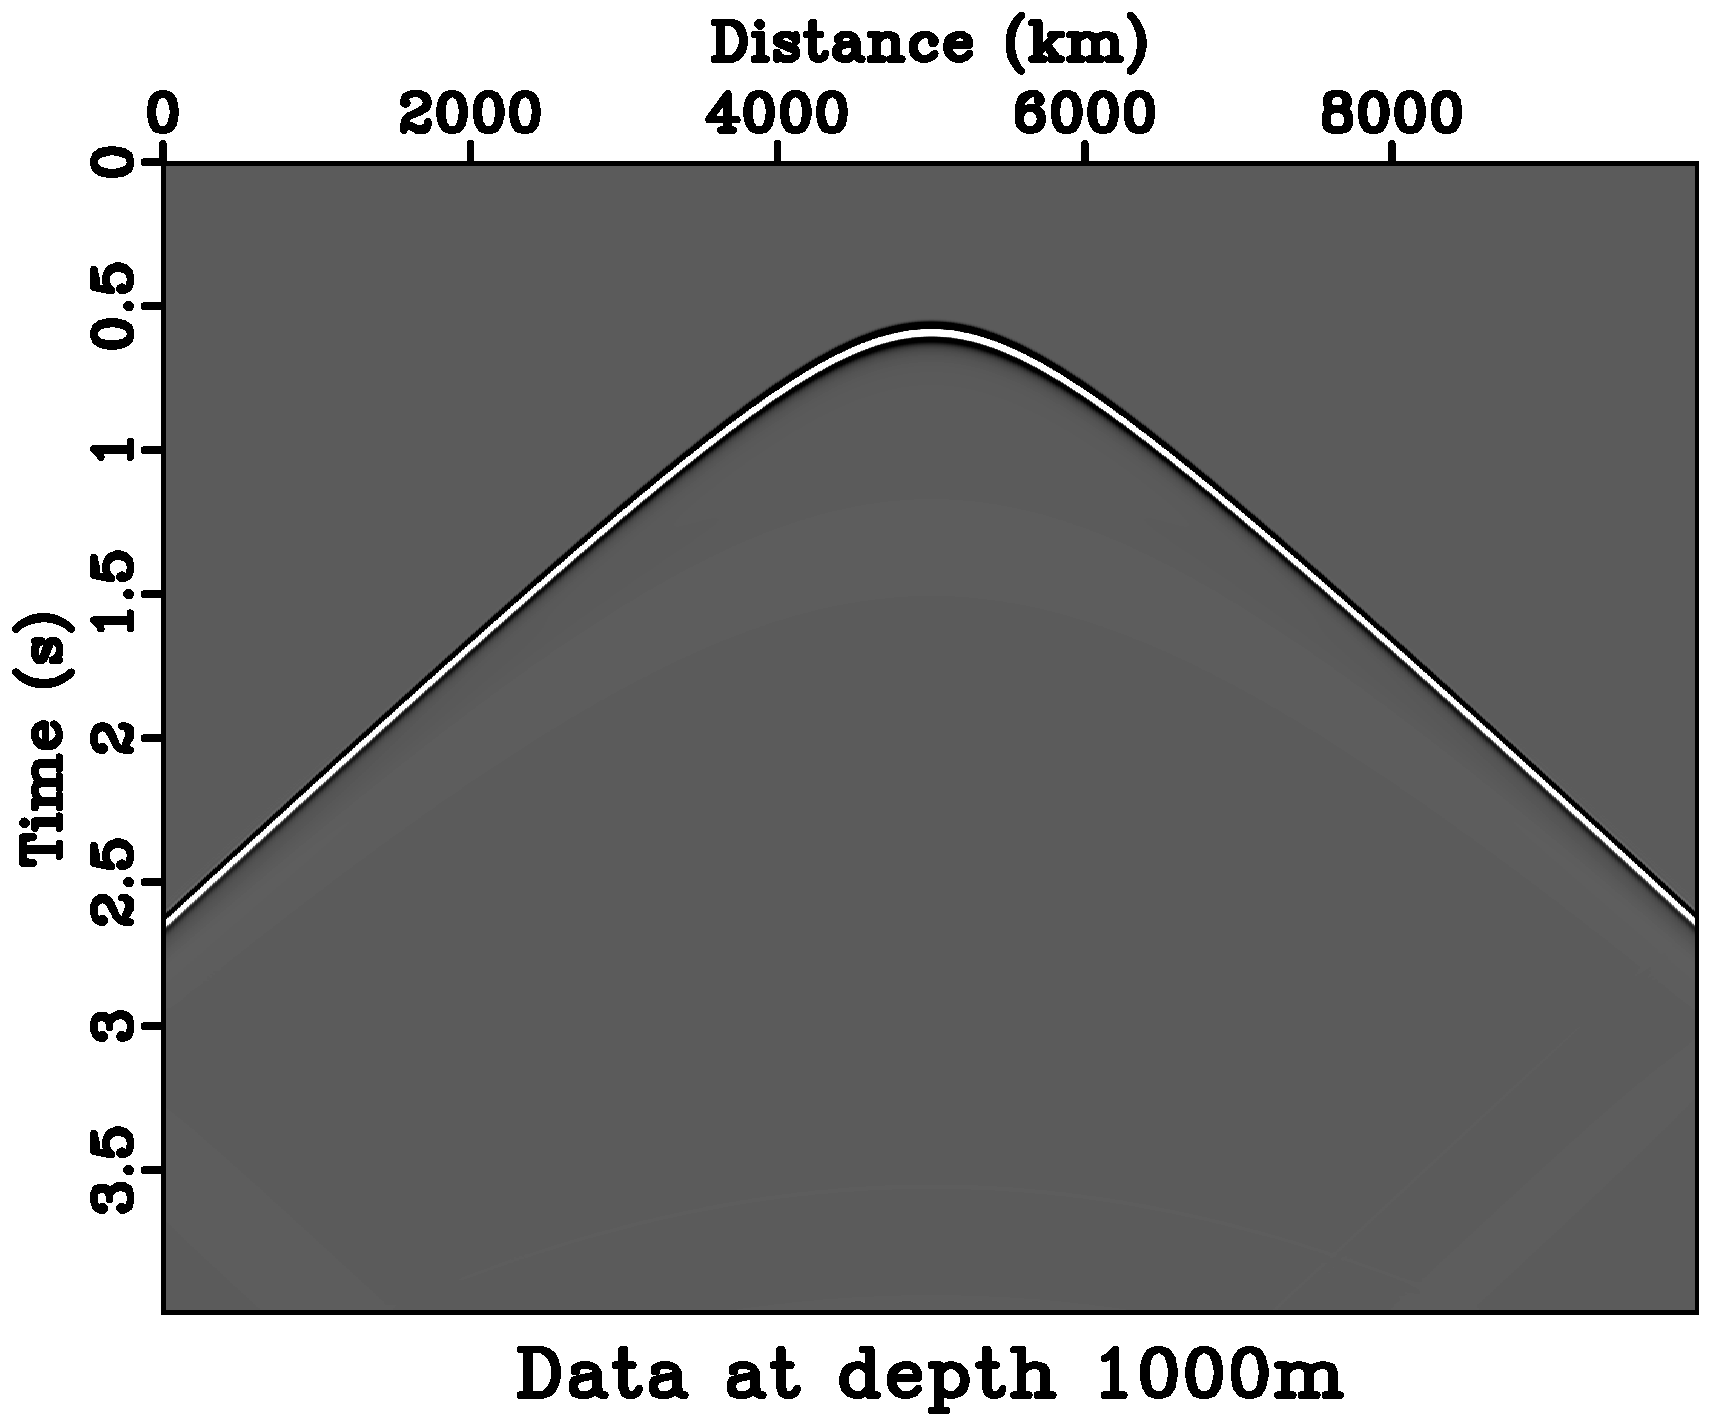
\epsfig{file=Fig/data-0-redat,width=8cm}
\end{figure}
\end{frame}
%-----------------------------------------
\begin{frame}{Imaging condition}
%-----------------------------------------
%
New imaging condition:
\begin{eqnarray}
  r(\xx,\xx',t=0)=
    \sum_{\xx_s}\int dt\,\d_z {p}_0(\xx,\xx_s,t)p_{sc}(\xx',\xx_s,t) 
\end{eqnarray}

Old imaging condition:
\begin{eqnarray}
    r_{c}(\xx,\xx',t=0)=\sum_{\xx_s}\int dt\, {p}_0(\xx,\xx_s,t)p_{sc}(\xx',\xx_s,t) 
\end{eqnarray}
%
\end{frame}
%-----------------------------------------
\begin{frame}{Numerical example}
%-----------------------------------------
Reflectivity $p_{sc}(\xx-\xx',t=0)$ at depth of 1000 m
using new imaging condition
%
\begin{figure}
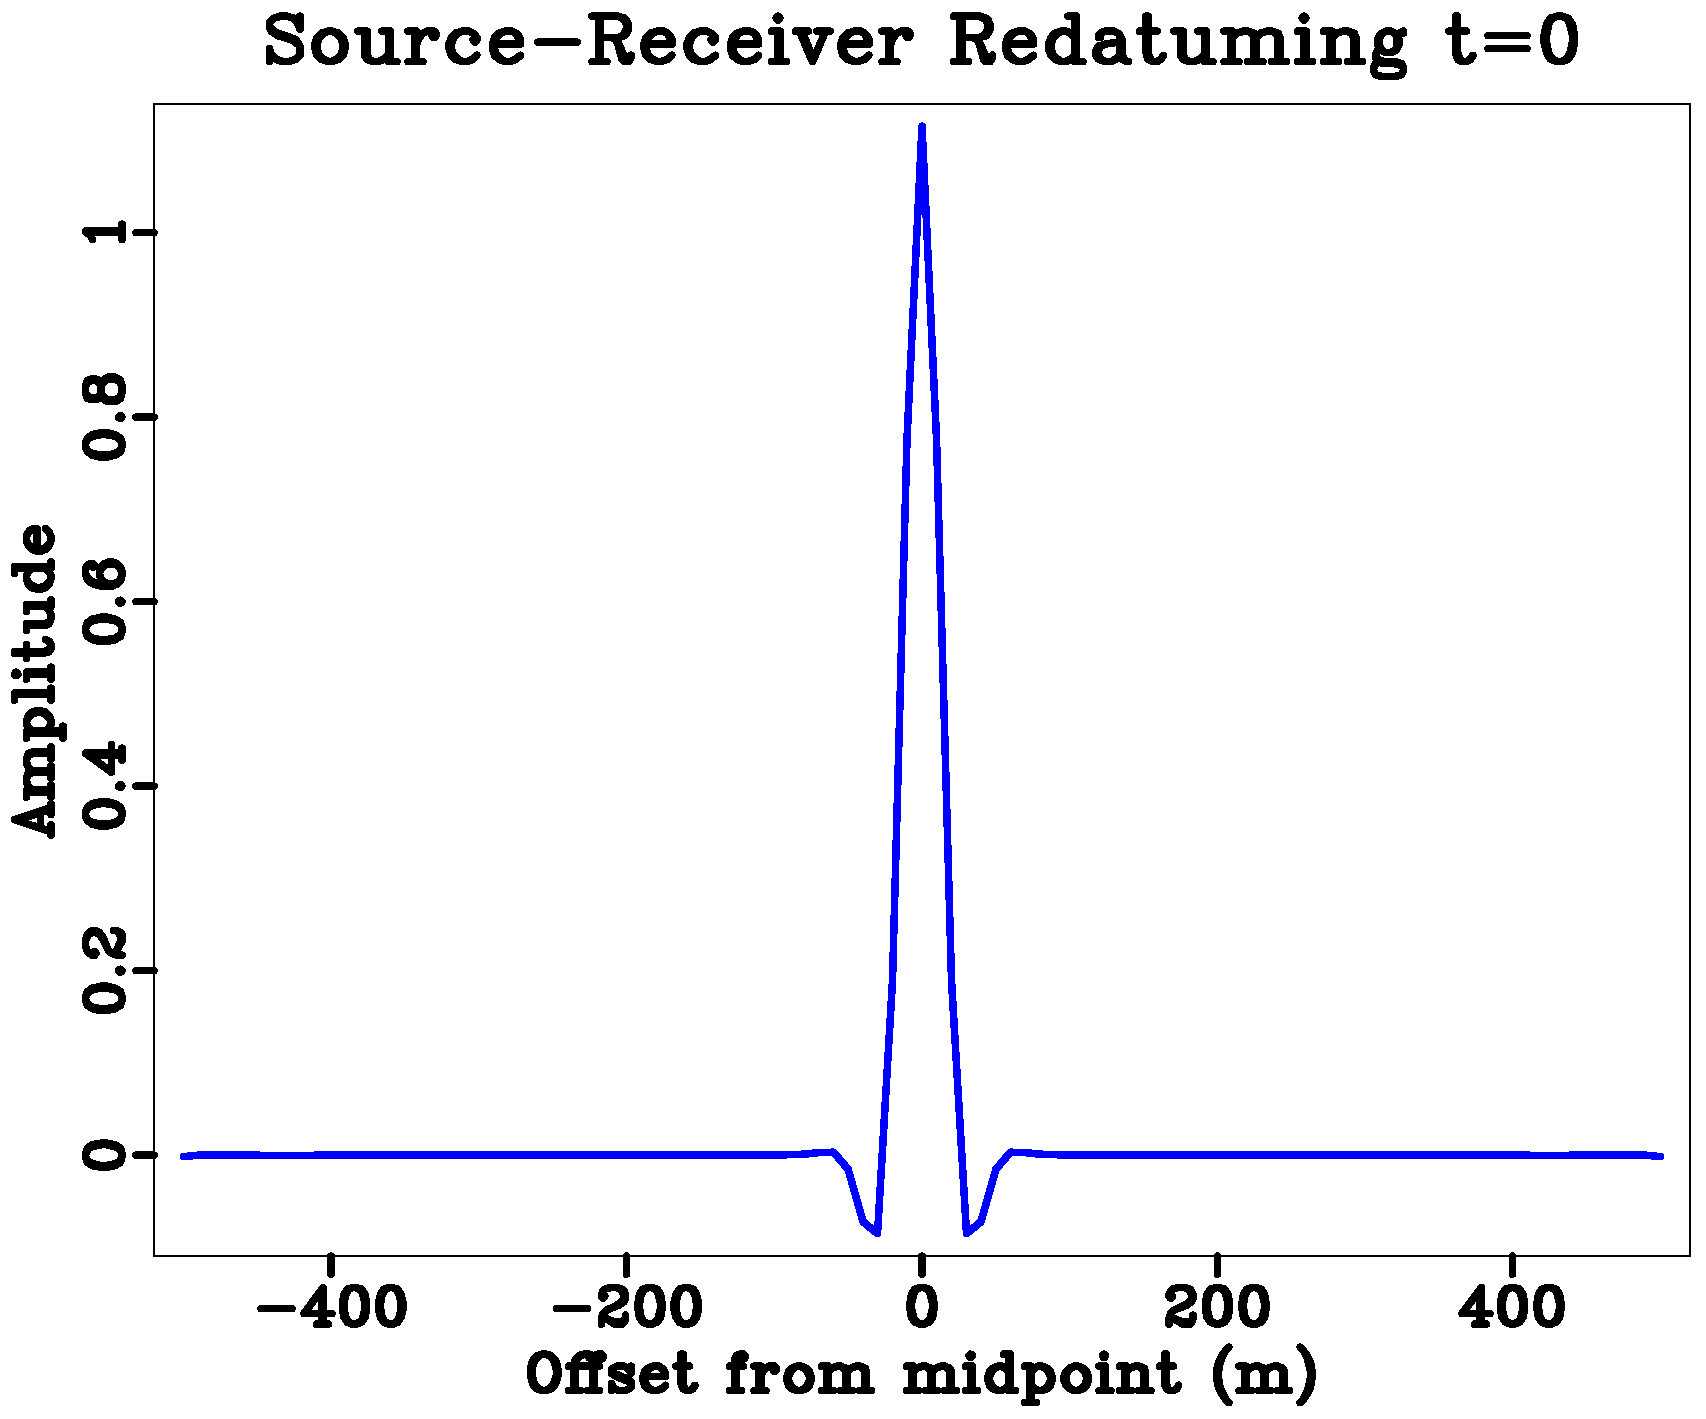
\epsfig{file=Fig/cip-1-ta-h-r1,width=8cm}
\end{figure}
\end{frame}
%-----------------------------------------
\begin{frame}{Numerical example}
%-----------------------------------------
%
Reflectivity $p_{sc}(\xx-\xx',t=0)$ at depth of 1000 m
using old imaging condition
\begin{figure}
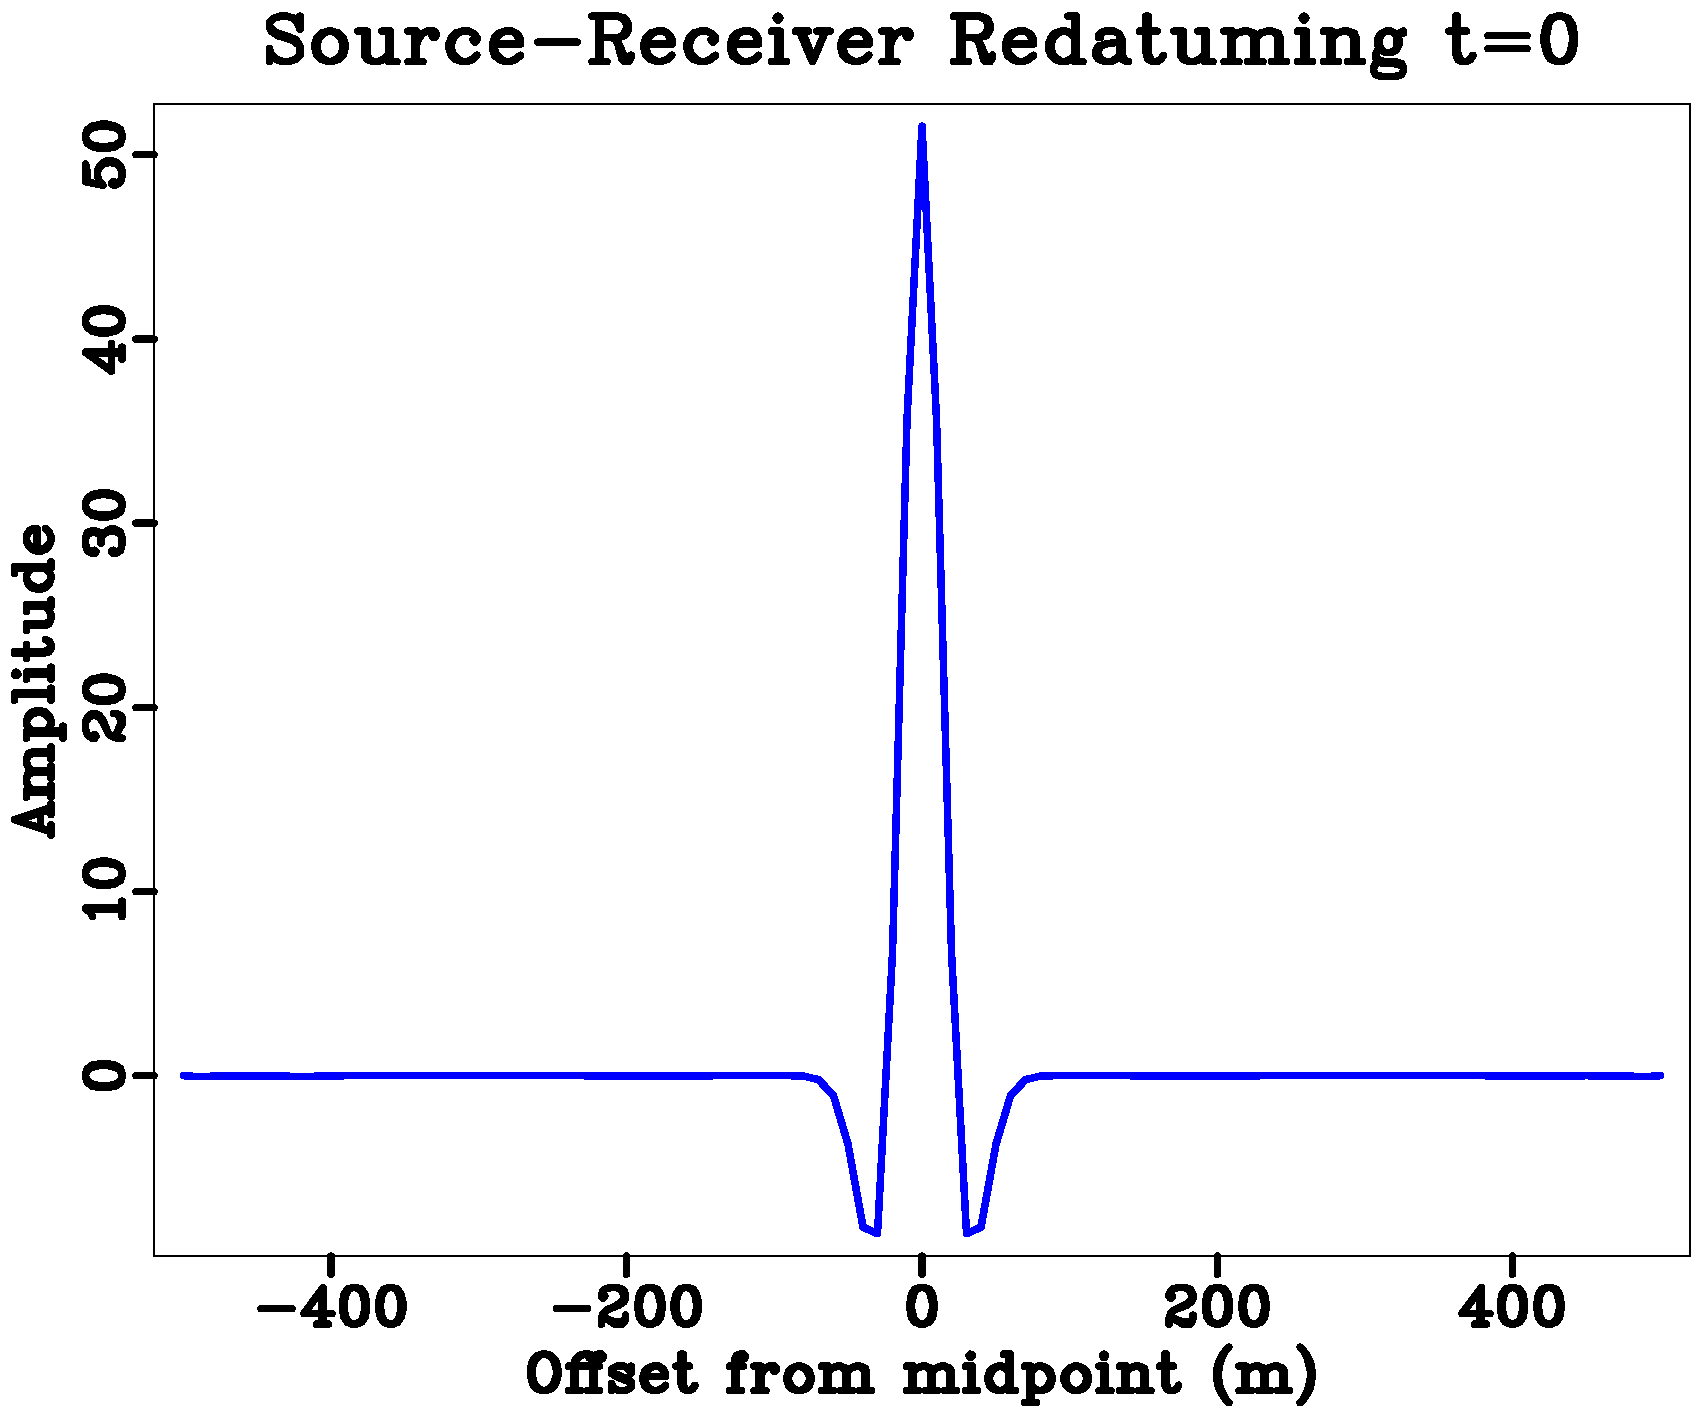
\epsfig{file=Fig/cip-1-cc-h-r1,width=8cm}
\end{figure}
\end{frame}
%-----------------------------------------
\begin{frame}{Numerical example}
%-----------------------------------------
Reflectivity $p_{sc}(\xx-\xx',t=0)$ at all depths
using new imaging condition
%
\begin{figure}
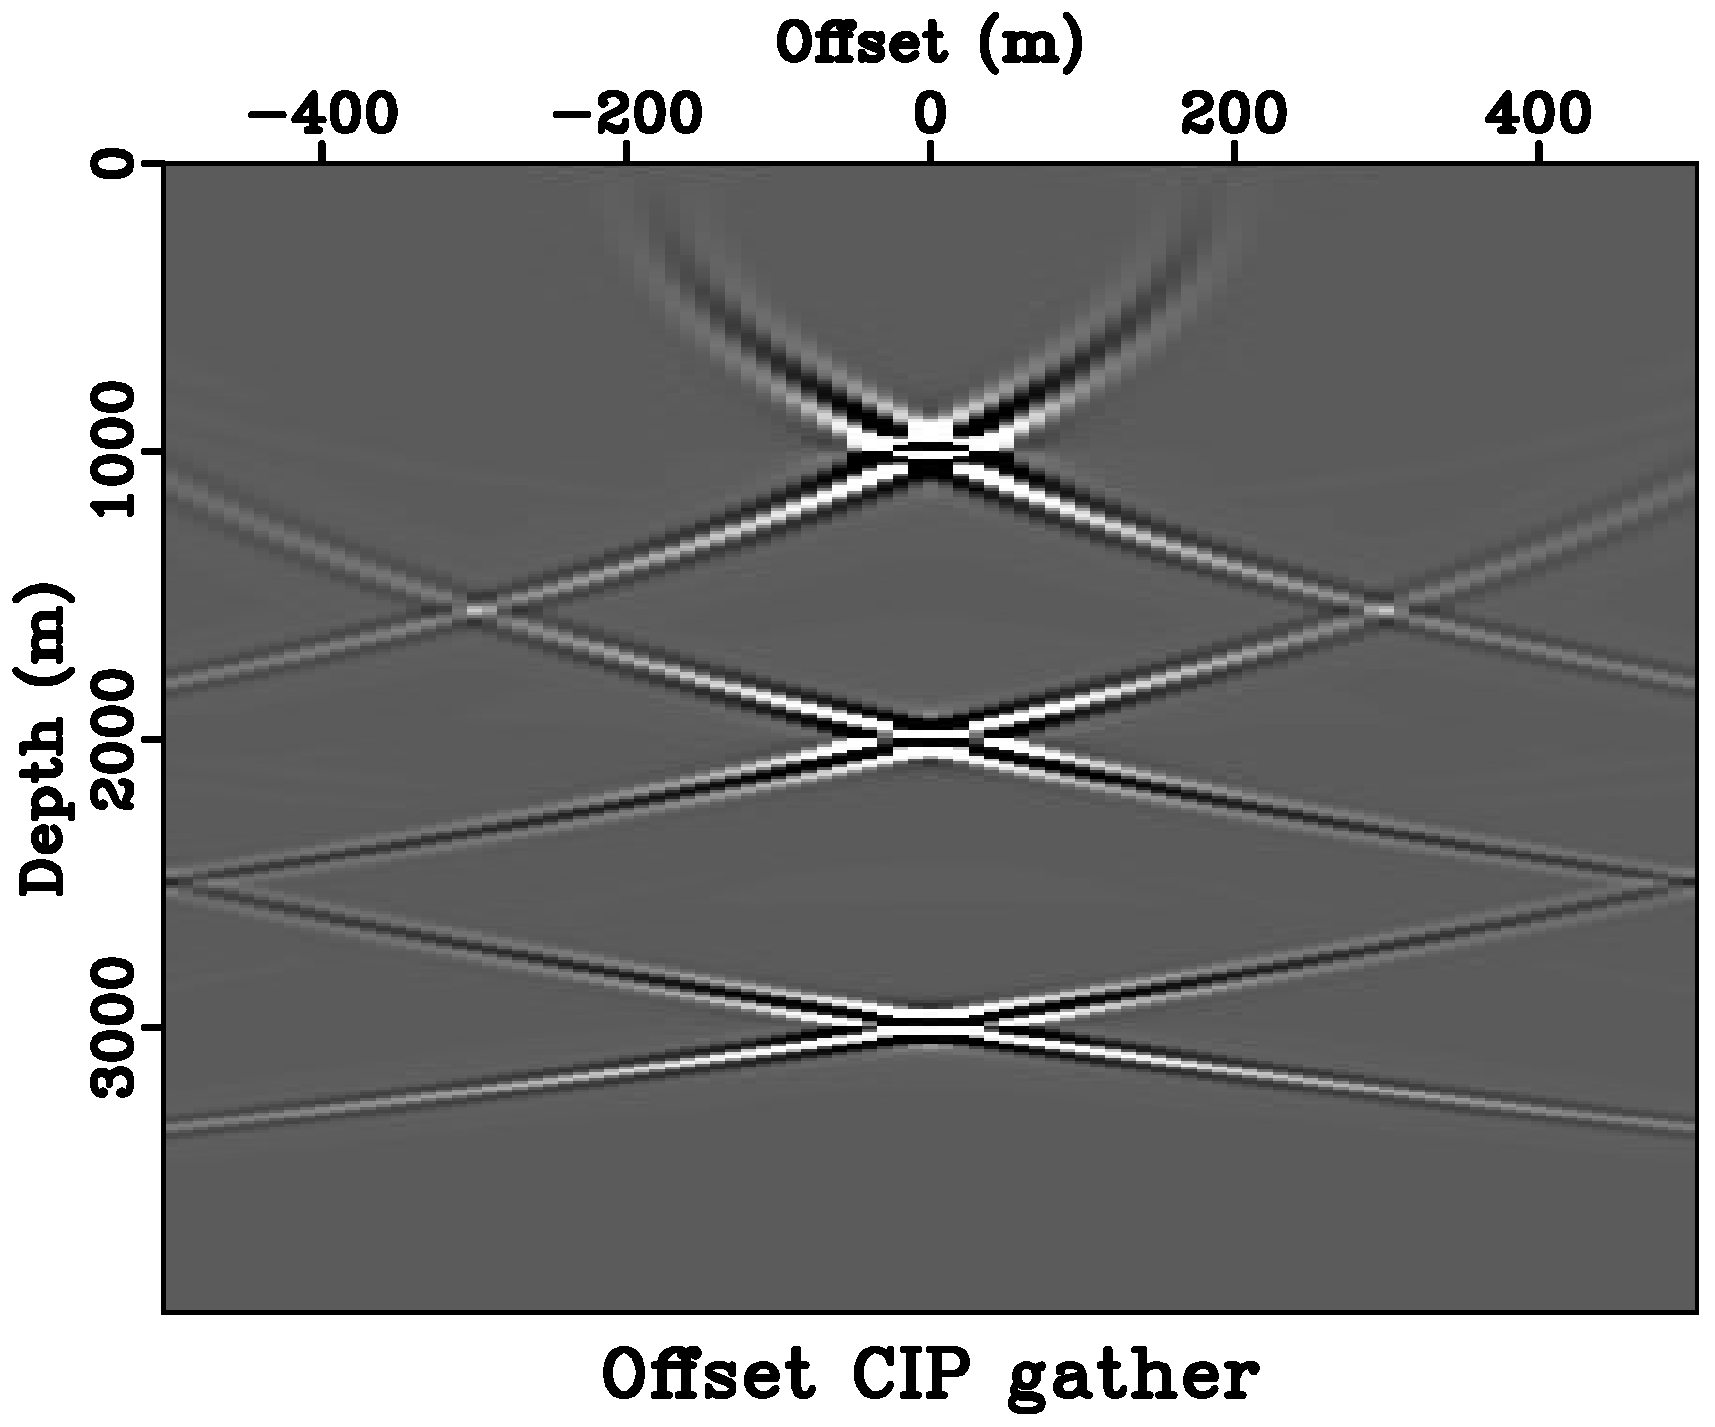
\epsfig{file=Fig/cip-1-ta,width=8cm}
\end{figure}
\end{frame}
%-----------------------------------------
\begin{frame}{Numerical example}
%-----------------------------------------
Full section $p_{sc}(\xx-\xx'=0,t)$ at all depths
using new imaging condition
%
\begin{figure}
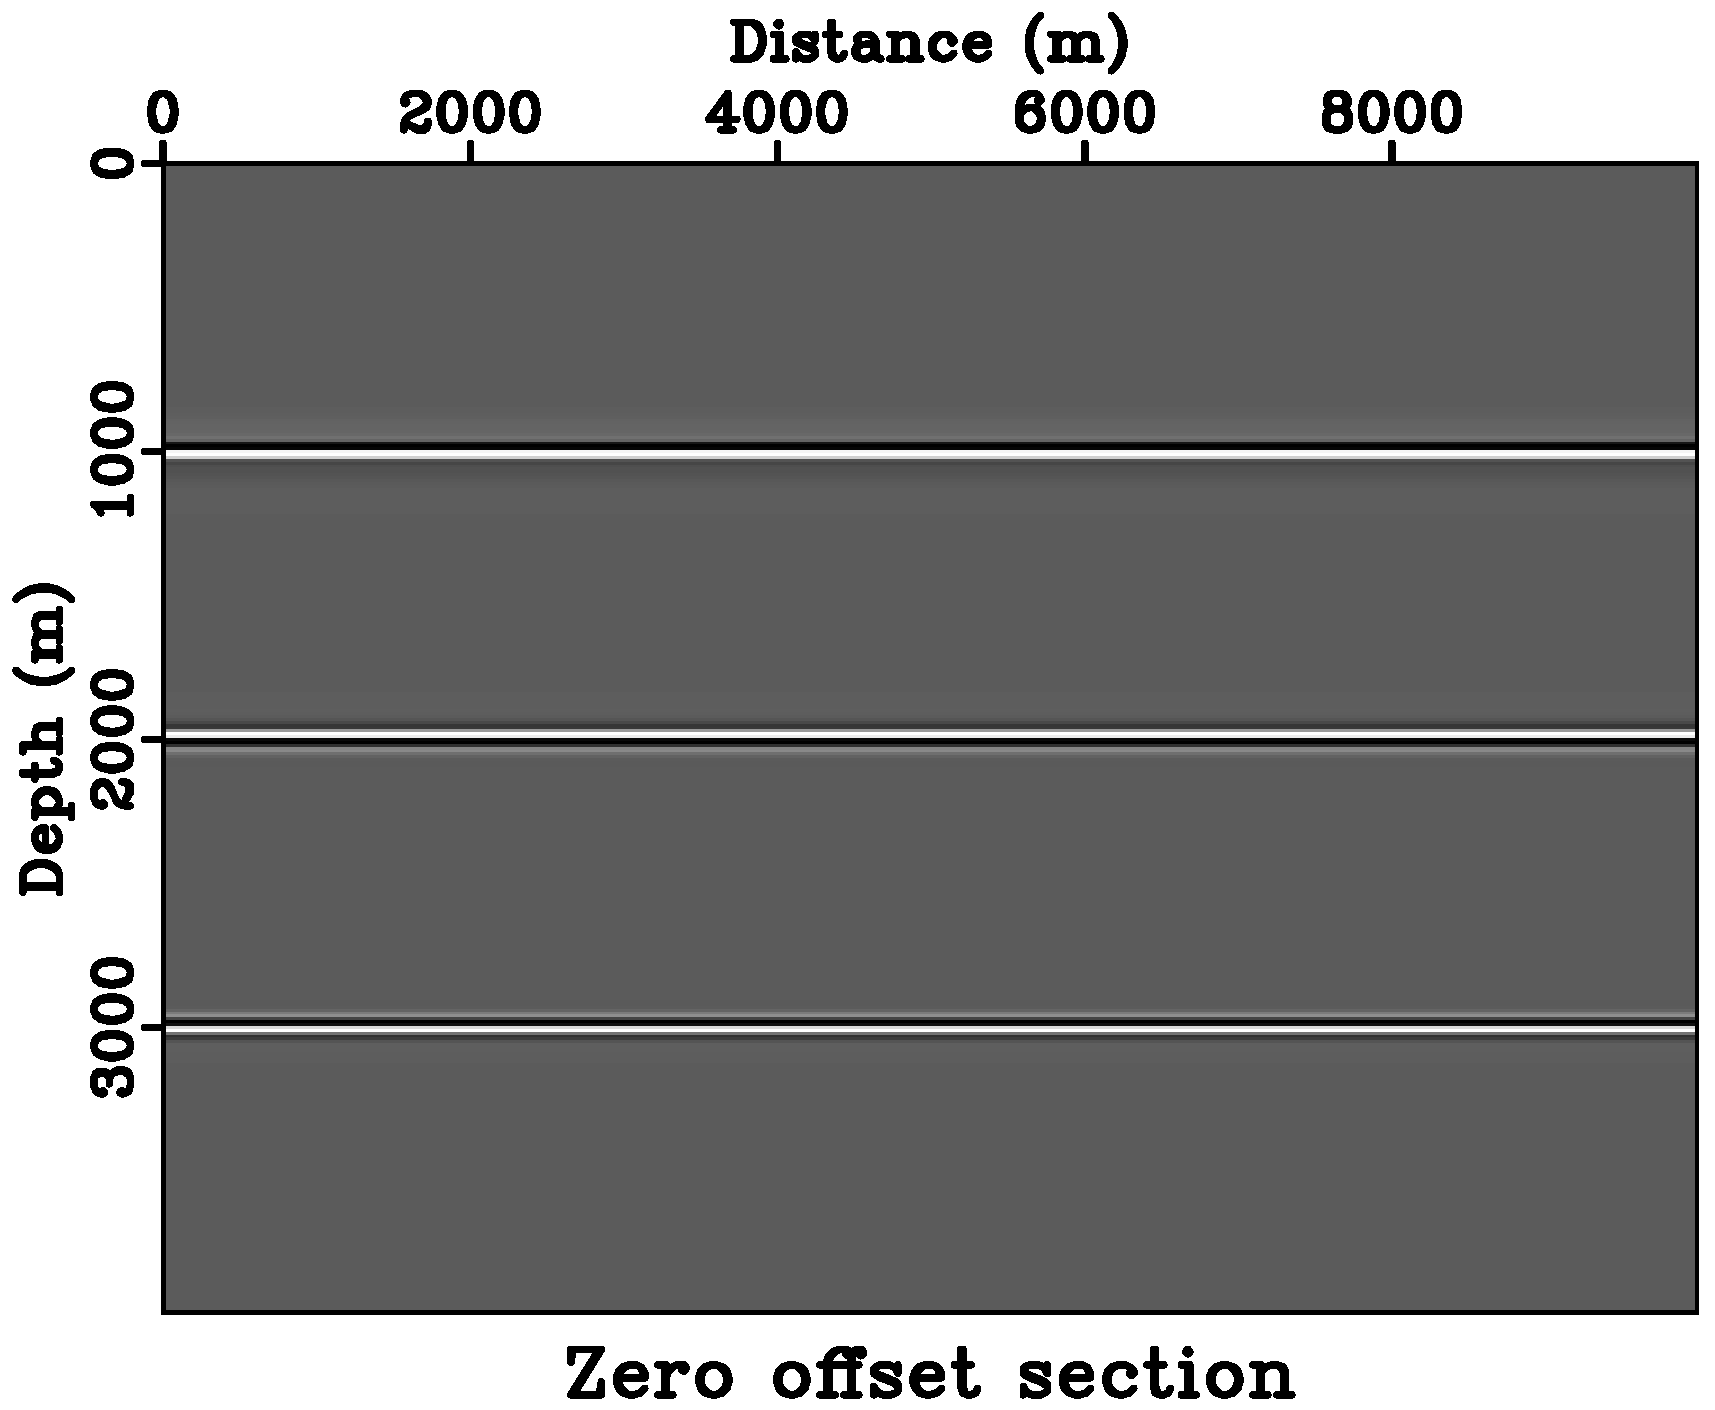
\epsfig{file=Fig/sect-ta,width=8cm}
\end{figure}
\end{frame}
%-----------------------------------------
\begin{frame}{Numerical example}
%-----------------------------------------
%
Plane wave reflection coefficient  $p_{sc}(\xx-\xx',t)$ at depth of 1000 m
using new imaging condition
\begin{figure}
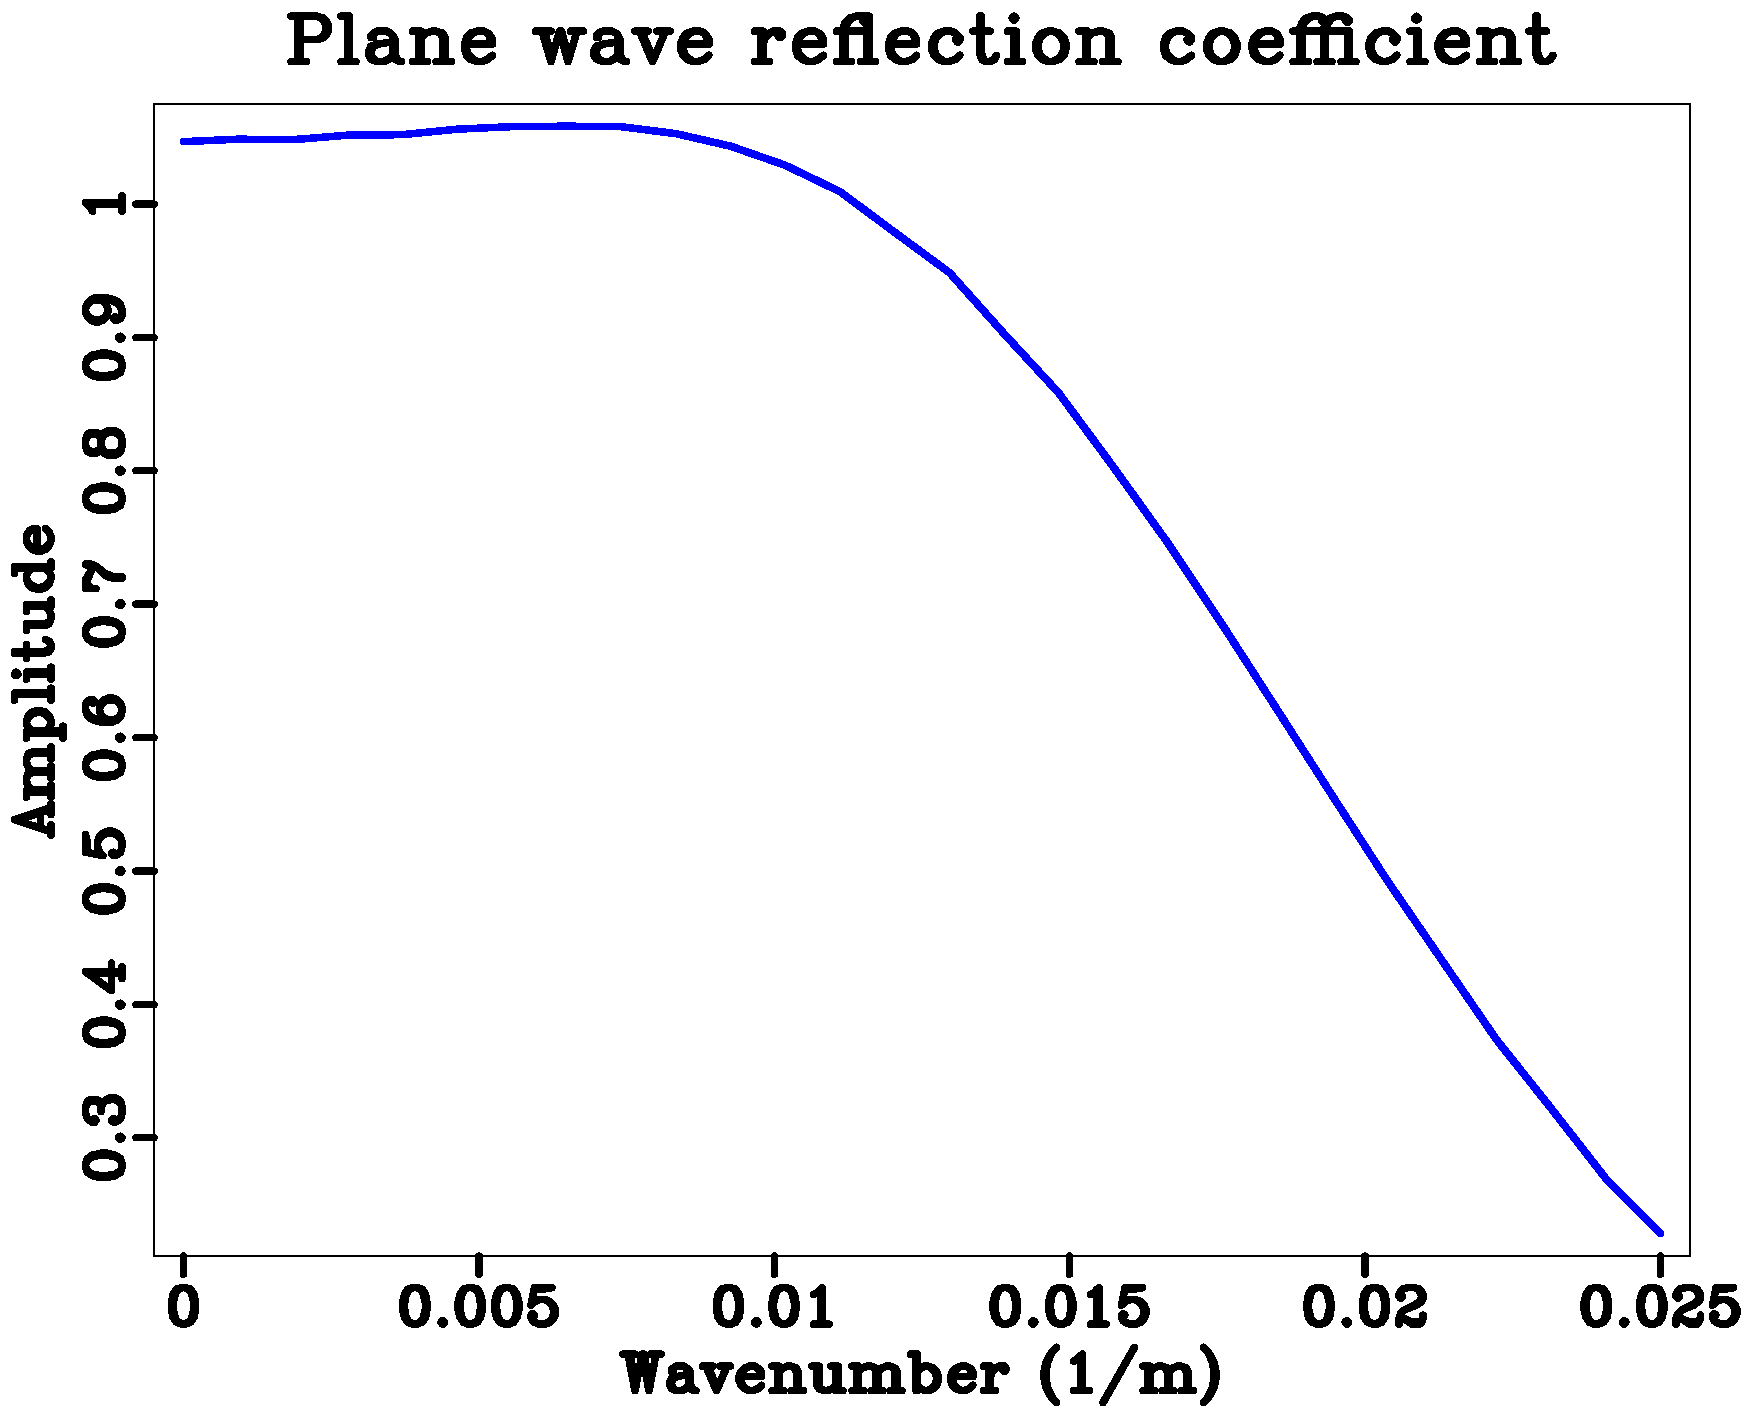
\epsfig{file=Fig/cip-1-ta-kx-r1,width=8cm}
\end{figure}
\end{frame}
%-----------------------------------------
\begin{frame}{Numerical example}
%-----------------------------------------
Plane wave reflection coefficient  $p_{sc}(\xx-\xx',t)$ at depth of 1000 m
using old imaging condition
%
\begin{figure}
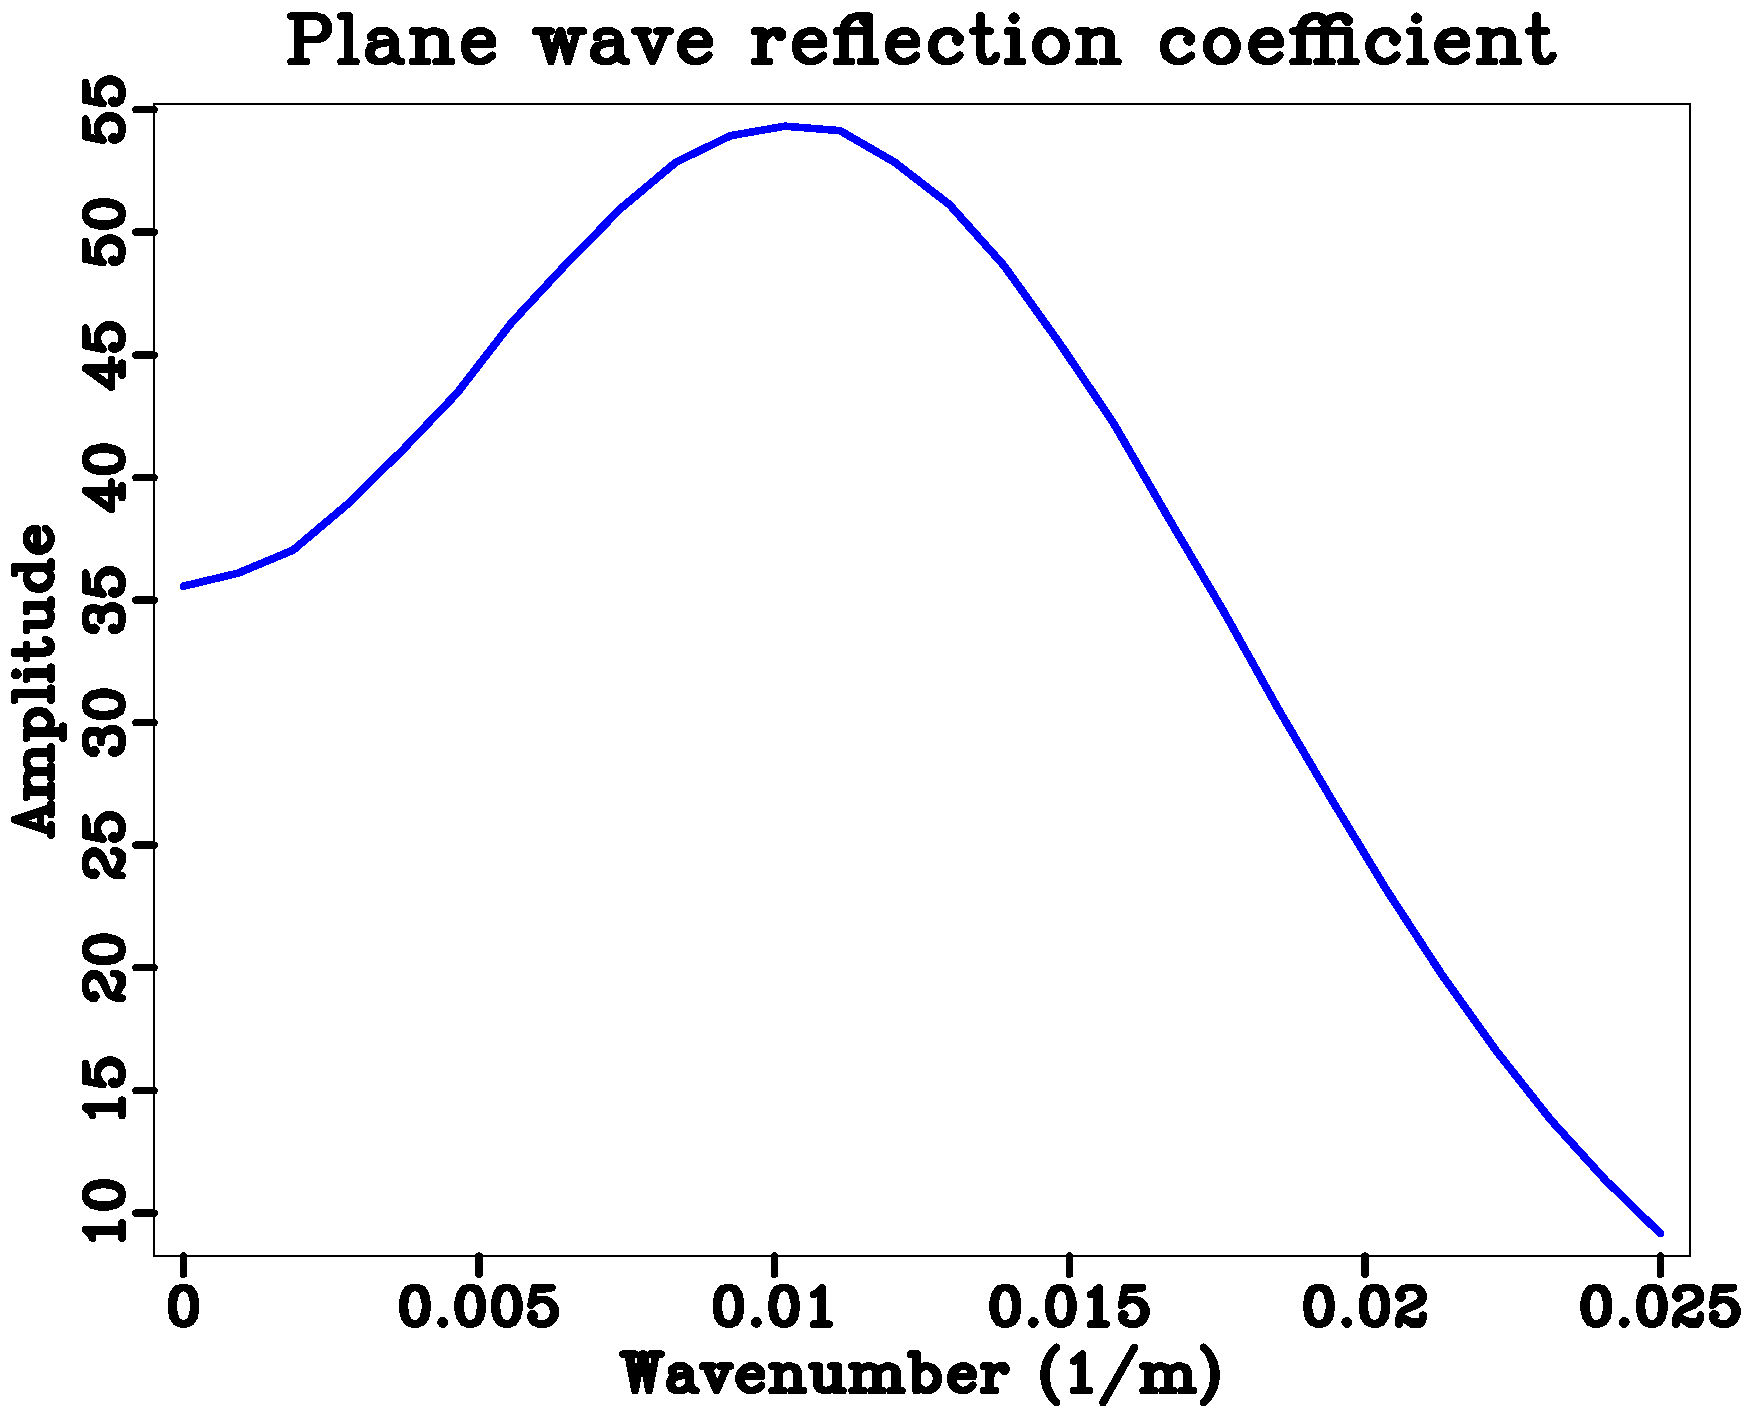
\epsfig{file=Fig/cip-1-cc-kx-r1,width=8cm}
\end{figure}
\end{frame}
%-----------------------------------------
\begin{frame}{Numerical example}
%-----------------------------------------
Reflection coefficient at three different depths
using new imaging condition
%
\begin{figure}
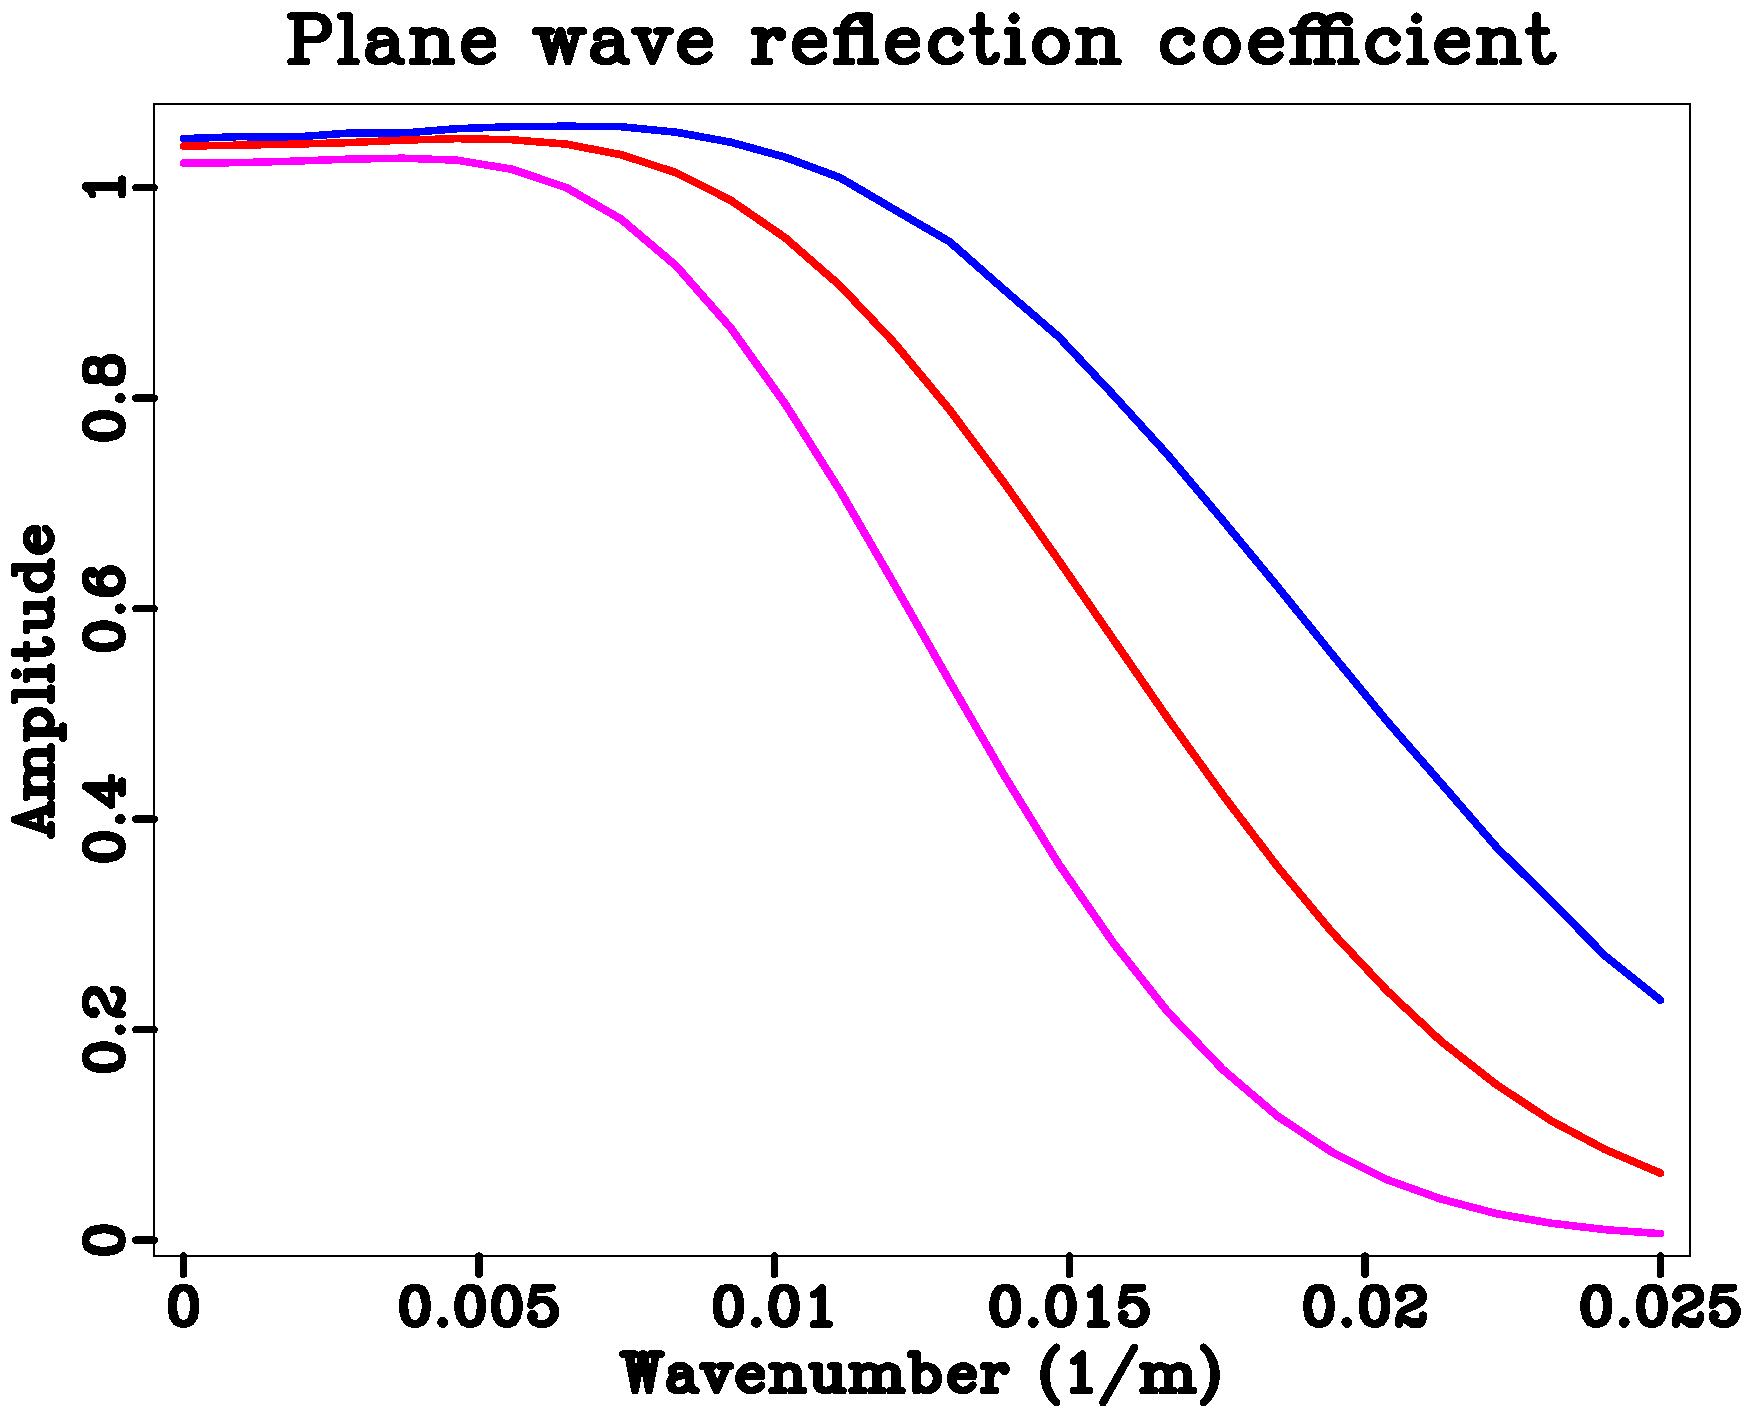
\epsfig{file=Fig/cip-1-ta-kx,width=8cm}
\end{figure}
\end{frame}
%-----------------------------------------
\begin{frame}{Numerical example}
%-----------------------------------------
%
Reflection coefficient at three different depths
using old imaging condition
\begin{figure}
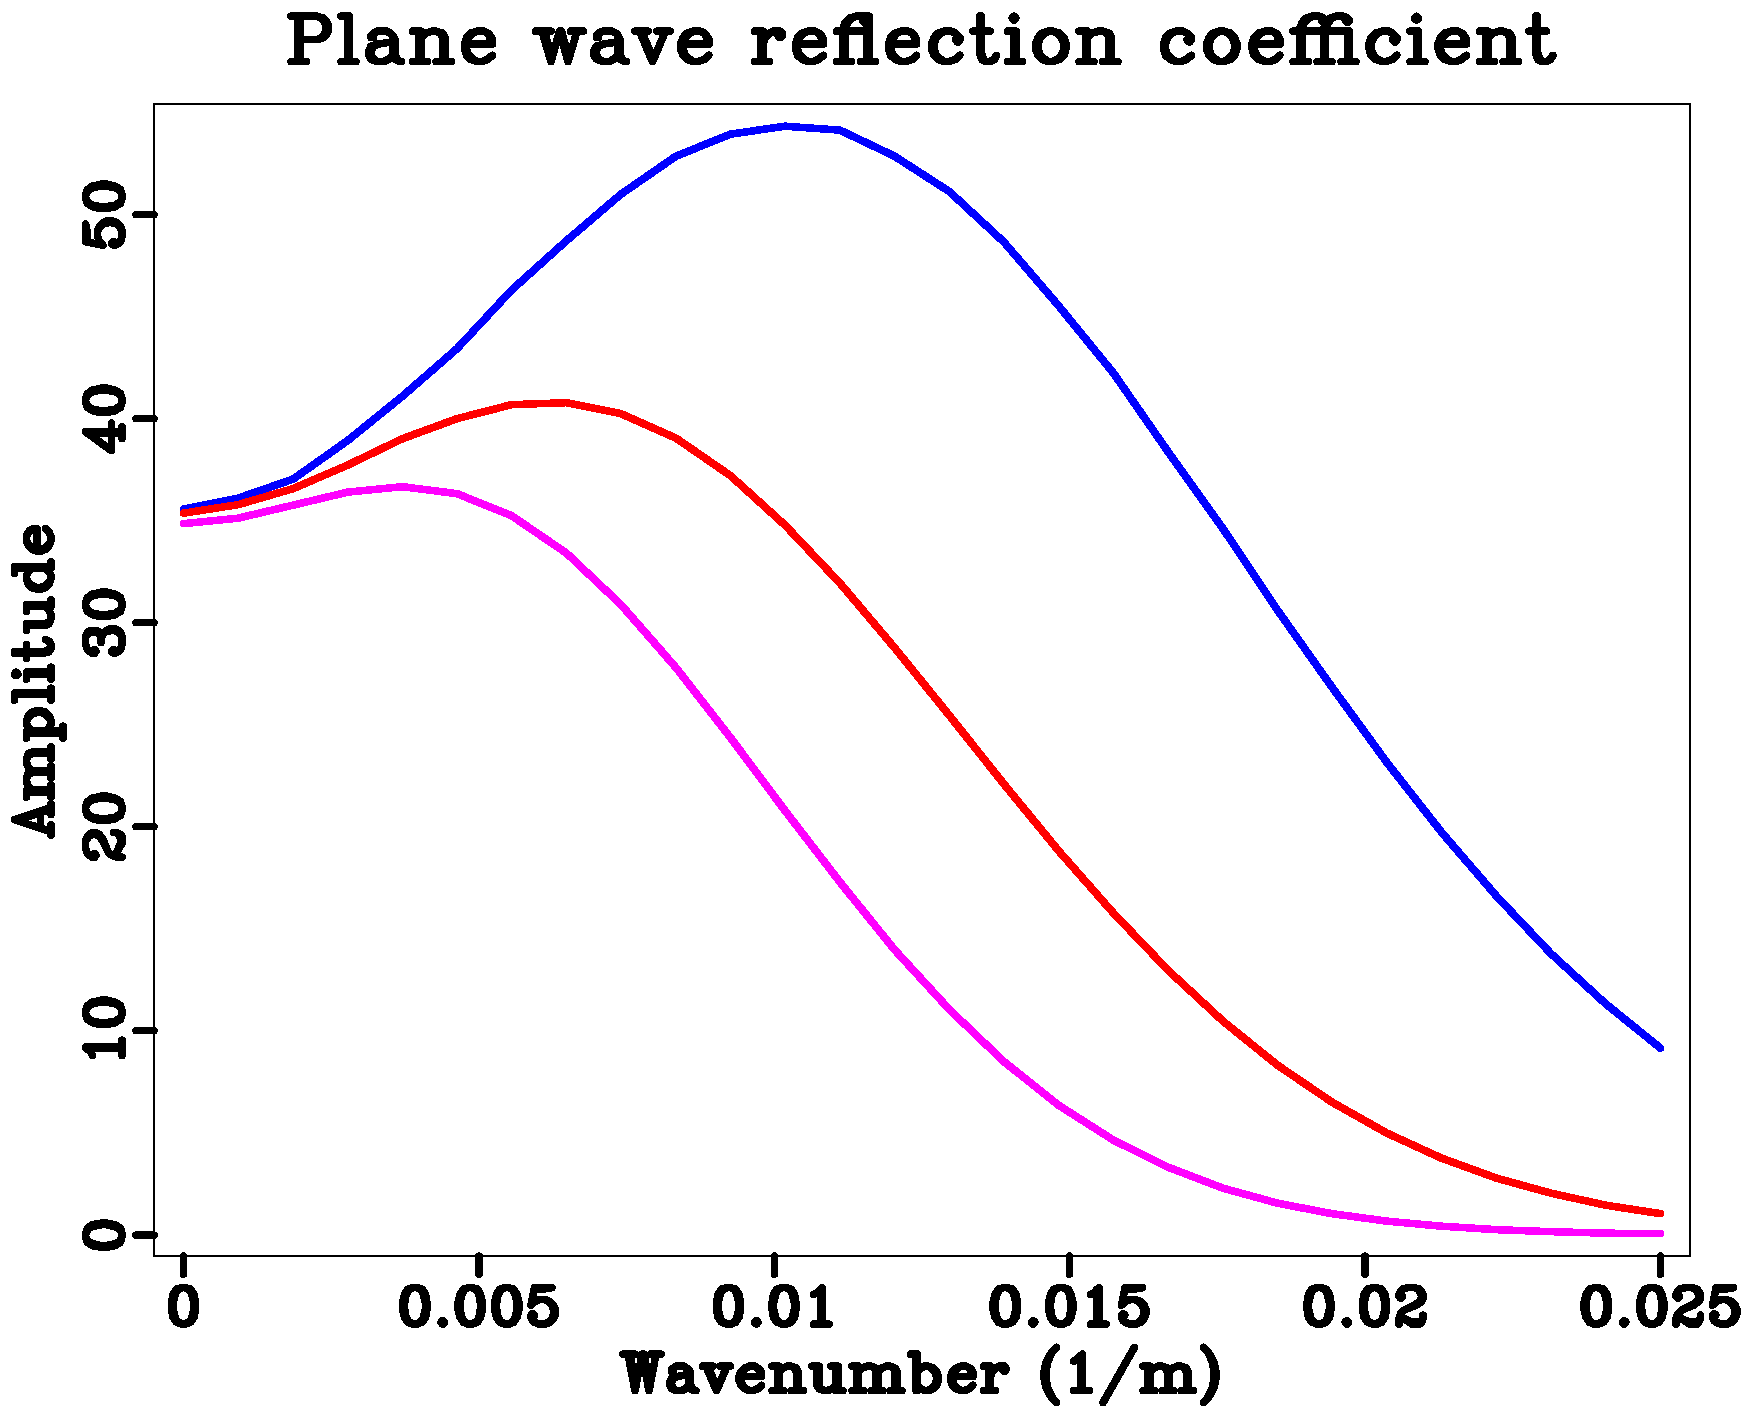
\epsfig{file=Fig/cip-1-cc-kx,width=8cm}
\end{figure}
\end{frame}
%-----------------------------------------
\begin{frame}{Summary/Conclusion}
%-----------------------------------------
%
\begin{itemize}
  \item New imaging condition gives correct Amplitude-Versus-Angle behaviour
  \item Easy to implement for reverse-time migration
  \item Simple modification of excisting imaging condition
\end{itemize}
\end{frame}
%-----------------------------------------
\begin{frame}{Imaging condition}
%-----------------------------------------
%
\begin{eqnarray}
  p_{sc}(\xx,\xx_s,t)=\
    -\int_S dS(\xx') \,  \rho^{-1}(\xx')\d_z p_{sc}(\xx',\xx_s,t)*\hat{g}(\xx,\xx',t) \nonumber\\
   + \int_S dS(\xx') \rho^{-1}(\xx')\d_z \hat{g}(\xx,\xx',t)*p_{sc}(\xx',\xx_s,t) 
\end{eqnarray}
%
%
\begin{eqnarray}
  p_{sc}(\xx,\xx_s,t)\approx
    \int_S dS(\xx') \rho^{-1}(\xx')2\d_z \hat{g}(\xx,\xx',t)*p_{sc}(\xx',\xx_s,t) 
\end{eqnarray}
%
\begin{itemize}
  \item $\hat{g}(\xx,\xx_s,t)$: Anticausal background Green's function
  \item $\rho$: Density
  \item $*$: Time convolution
\end{itemize}
\end{frame}
%-----------------------------------------
\begin{frame}{Imaging condition}
%-----------------------------------------
%
\begin{eqnarray}
  p_{sc}(\xx,\xx',t)*\hat{s}(t)=\
    -  \int_S dS(\xx_s) \rho^{-1}(\xx_s)\, \d_z p_{sc}(\xx',\xx_s,t)*\hat{p}_0(\xx,\xx_s,t) \nonumber\\
   + \int_S ds(\xx_s) \d_z \hat{p}_0(\xx',\xx_s,t)*p_{sc}(\xx',\xx_s,t) 
\end{eqnarray}
%
%
\begin{eqnarray}
  p_{sc}(\xx,\xx',t)*\hat{s}(t) \approx
    \int_S ds(\xx_s) \d_z \hat{p}_0(\xx',\xx_s,t)*p_{sc}(\xx',\xx_s,t) 
\end{eqnarray}
%
\begin{itemize}
  \item $\hat{p}_0(\xx,\xx_s,t)$: Anticausal downgoing wavefield 
\end{itemize}
\end{frame}
\end{document}
